\documentclass[11pt]{beamer}
\usepackage{xcolor}
\graphicspath{{Images/}{./}} % Specifies where to look for included images (trailing slash required)
\usepackage{graphics}
%\addmediapath{/Users/hoangleson/Documents/Lecture in University /DHQG/DHQG-DuocLieu/Movies}
\usepackage[utf8]{vietnam}
\usepackage{ragged2e}
\apptocmd{\frame}{}{\justifying}{}
\usepackage{booktabs}
\usepackage{multirow}
\usepackage{booktabs}
\usepackage{setspace}
\usepackage{fancybox}
\usepackage{multimedia}
\usepackage[caption=false]{subfig}
\usepackage[librsvg]{chemobabel}
\usepackage{chemfig}
\usepackage{pdfpages}
% Beamer comes with a number of default layout themes which change the colors and layouts of slides. Below is a list of all themes available, uncomment each in turn to see what they look like.

%\usetheme{default}
%\usetheme{AnnArbor}
%\usetheme{Antibes}
%\usetheme{Bergen}
%\usetheme{Berkeley}
%\usetheme{Berlin}
%\usetheme{Boadilla}
%\usetheme{CambridgeUS}
%\usetheme{Copenhagen}
%\usetheme{Darmstadt}
%\usetheme{Dresden}
%\usetheme{Frankfurt}
%\usetheme{Goettingen}
%\usetheme{Hannover}
%\usetheme{Ilmenau}
%\usetheme{JuanLesPins}
%\usetheme{Luebeck}
%\usetheme{Madrid}
%\usetheme{Malmoe}
%\usetheme{Marburg}
%\usetheme{Montpellier}
%\usetheme{PaloAlto}
%\usetheme{Pittsburgh}
%\usetheme{Rochester}
%\usetheme{Singapore}
%\usetheme{Szeged}
%\usetheme{Warsaw}
%\usetheme{SimpleDarkBlue}

%----------------------------------------------------------------------------------------
%	SELECT COLOR THEME
%----------------------------------------------------------------------------------------

% Beamer comes with a number of color themes that can be applied to any layout theme to change its colors. Uncomment each of these in turn to see how they change the colors of your selected layout theme.

%\usecolortheme{albatross}
%\usecolortheme{beaver}
%\usecolortheme{beetle}
%\usecolortheme{crane}
%\usecolortheme{dolphin}
%\usecolortheme{dove}
%\usecolortheme{fly}
%\usecolortheme{lily}
%\usecolortheme{monarca}
%\usecolortheme{seagull}
%\usecolortheme{seahorse}
%\usecolortheme{spruce}
%\usecolortheme{whale}
%\usecolortheme{wolverine}
%----------------------------------------------------------------------------------------
%	SELECT FONT THEME & FONTS
%----------------------------------------------------------------------------------------

% Beamer comes with several font themes to easily change the fonts used in various parts of the presentation. Review the comments beside each one to decide if you would like to use it. Note that additional options can be specified for several of these font themes, consult the beamer documentation for more information.

\usefonttheme{default} % Typeset using the default sans serif font
%\usefonttheme{serif} % Typeset using the default serif font (make sure a sans font isn't being set as the default font if you use this option!)
%\usefonttheme{structurebold} % Typeset important structure text (titles, headlines, footlines, sidebar, etc) in bold
%\usefonttheme{structureitalicserif} % Typeset important structure text (titles, headlines, footlines, sidebar, etc) in italic serif
%\usefonttheme{structuresmallcapsserif} % Typeset important structure text (titles, headlines, footlines, sidebar, etc) in small caps serif

%------------------------------------------------

%\usepackage{mathptmx} % Use the Times font for serif text
\usepackage{palatino} % Use the Palatino font for serif text

%\usepackage{helvet} % Use the Helvetica font for sans serif text
%\usepackage[default]{opensans} % Use the Open Sans font for sans serif text
%\usepackage[default]{FiraSans} % Use the Fira Sans font for sans serif text
%\usepackage[default]{lato} % Use the Lato font for sans serif text

%----------------------------------------------------------------------------------------
%	SELECT INNER THEME
%----------------------------------------------------------------------------------------

% Inner themes change the styling of internal slide elements, for example: bullet points, blocks, bibliography entries, title pages, theorems, etc. Uncomment each theme in turn to see what changes it makes to your presentation.

%\useinnertheme{default}
%\useinnertheme{circles}
%\useinnertheme{rectangles}
%\useinnertheme{rounded}
%\useinnertheme{inmargin}

%----------------------------------------------------------------------------------------
%	SELECT OUTER THEME
%----------------------------------------------------------------------------------------

% Outer themes change the overall layout of slides, such as: header and footer lines, sidebars and slide titles. Uncomment each theme in turn to see what changes it makes to your presentation.
%\setbeamertemplate{headline}{}
%\useoutertheme{default}
\useoutertheme{infolines}
%\useoutertheme{miniframes}
%\useoutertheme{smoothbars}
%\useoutertheme{sidebar}
%\useoutertheme{split}
%\useoutertheme{shadow}
%\useoutertheme{tree}
%\useoutertheme{smoothtree}

%\setbeamertemplate{footline} % Uncomment this line to remove the footer line in all slides
\setbeamertemplate{footline}[page number] % Uncomment this line to replace the footer line in all slides with a simple slide count
\setbeamertemplate{caption}{\raggedright\insertcaption\par}
%\setbeamertemplate{navigation symbols}{} % Uncomment this line to remove the navigation symbols from the bottom of all slides

%----------------------------------------------------------------------------------------
%	PRESENTATION INFORMATION
%----------------------------------------------------------------------------------------

\title[Dược Liệu]{DƯỢC LIỆU CHỨA FLAVONOIDS} % The short title in the optional parameter appears at the bottom of every slide, the full title in the main parameter is only on the title page

%\subtitle{Dược liệu và các hợp chất từ tự nhiên} % Presentation subtitle, remove this command if a subtitle isn't required

\author[PhD. Hoàng Lê Sơn]{} % Presenter name(s), the optional parameter can contain a shortened version to appear on the bottom of every slide, while the main parameter will appear on the title slide

%\institute[UC]{Bộ môn Dược liệu \\ \smallskip \textit{hoangson.med@gmail.com}} % Your institution, the optional parameter can be used for the institution shorthand and will appear on the bottom of every slide after author names, while the required parameter is used on the title slide and can include your email address or additional information on separate lines
\usepackage{tikz}
\usetikzlibrary{trees}
%\titlegraphic { 
%\begin{tikzpicture}[overlay,remember picture]
%\node [xshift=0cm,yshift=4cm] at (current page.center){
%    
\includegraphics[width=1.2cm]{Logo.jpg}
%};
%\end{tikzpicture}
%}




\date[\today]{\tiny\today} % Presentation date or conference/meeting name, the optional parameter can contain a shortened version to appear on the bottom of every slide, while the required parameter value is output to the title slide

%----------------------------------------------------------------------------------------
\definecolor{InvisibleRed}{rgb}{0.92, 0.9, 0.9}
\definecolor{InvisibleGreen}{rgb}{0.9, 0.92, 0.9}
\definecolor{InvisibleBlue}{rgb}{0.9, 0.9, 0.92}
\definecolor{LightBlue}{rgb}{0.4, 0.55, 0.65}
\definecolor{MediumRed}{rgb}{0.92549, 0.34509, 0.34509}
\definecolor{MediumGreen}{rgb}{0.36862, 0.66666, 0.65882}
\definecolor{MediumBlue}{rgb}{0.01176, 0.31372, 0.43529}
\definecolor{DarkBlue}{rgb}{0.05, 0.15, 0.3} 
\definecolor{ColorDN}{rgb}{1, 0.39, 0.28} 
\setbeamercovered{transparent}
\usepackage{tikz}
\usetikzlibrary{overlay-beamer-styles}
 \tikzset{
    highlight on/.style={alt={#1{fill=red!80!black,color=red!80!black}{fill=gray!30!white,color=gray!30!white}}},
}
\usepackage{chronology}
\usepackage{blindtext}
\setbeamertemplate{navigation symbols}{}
\setbeamerfont{caption}{size=\scriptsize}
\setbeamercolor{palette primary}{bg=DarkBlue,fg=white}
\setbeamercolor{palette secondary}{bg=MediumBlue,fg=white}
\setbeamercolor{palette tertiary}{bg=LightBlue,fg=white}
\setbeamercolor{block title}{bg=ColorDN,fg=white}
\setbeamercolor{block body}{bg=InvisibleBlue}
\setbeamercolor{part title}{fg=white, bg=black}
\setbeamerfont{block title}{size=\normalfont,series=\mdseries,parent={structure,block body}}
\setbeamerfont{block body}{size=\small}
\setbeamertemplate{headline}{}
\setbeamercolor*{frametitle}{bg=white}
\makeatletter
\setbeamertemplate{frametitle}{%
  \ifbeamercolorempty[bg]{frametitle}{}{\nointerlineskip}%
  \@tempdima=\textwidth%
  \advance\@tempdima by\beamer@leftmargin%
  \advance\@tempdima by\beamer@rightmargin%
  \advance\@tempdima by-3cm% <- change value here
  \hfill%
  \begin{beamercolorbox}[sep=0.4cm,left,wd=\the\@tempdima]{frametitle}
    \usebeamerfont{frametitle}%
    \vbox{}\vskip-1ex%
    \if@tempswa\else\csname beamer@fteleft\endcsname\fi%
    \strut\insertframetitle\strut\par%
    {%
      \ifx\insertframesubtitle\@empty%
      \else%
      {\usebeamerfont{framesubtitle}\usebeamercolor[fg]{framesubtitle}\strut\insertframesubtitle\strut\par}%
      \fi
    }%
    \vskip-1ex%
    \if@tempswa\else\vskip-.3cm\fi% set inside beamercolorbox... evil here...
  \end{beamercolorbox}%
}
\makeatother
\makeatletter
\def\parsecomma#1,#2\endparsecomma{\def\page@x{#1}\def\page@y{#2}}
\tikzdeclarecoordinatesystem{page}{
    \parsecomma#1\endparsecomma
    \pgfpointanchor{current page}{north east}
    % Save the upper right corner
    \pgf@xc=\pgf@x%
    \pgf@yc=\pgf@y%
    % save the lower left corner
    \pgfpointanchor{current page}{south west}
    \pgf@xb=\pgf@x%
    \pgf@yb=\pgf@y%
    % Transform to the correct placement
    \pgfmathparse{(\pgf@xc-\pgf@xb)/2.*\page@x+(\pgf@xc+\pgf@xb)/2.}
    \expandafter\pgf@x\expandafter=\pgfmathresult pt
    \pgfmathparse{(\pgf@yc-\pgf@yb)/2.*\page@y+(\pgf@yc+\pgf@yb)/2.}
    \expandafter\pgf@y\expandafter=\pgfmathresult pt
}
\makeatother

\newcommand{\mysectionpage}{
    \begingroup
    \setbeamertemplate{background}{
		
\includegraphics[width=\paperwidth,height=\paperheight]{Bia2.pdf}
    }
	\setbeamercolor{section page}{fg=DarkBlue}
    \setbeamertemplate{section page}{
	\centering
	\usebeamerfont{title}\insertsectionhead\par
    }
    \frame{\sectionpage}
    \endgroup
}

\begin{document}




%-------------------------------------------------------------------------------

%	TITLE SLIDE

\begin{frame}[plain]
	\begin{tikzpicture}[remember picture,overlay]
	% Background image
		\node[above right] at (current page.south west)
		{
			
\includegraphics[width=\paperwidth,height=\paperheight]{Bia1.pdf}
		};
		
	% Title & Subtitle
	\node
	[
		%above=-1cm,
		align=center,
		fill=LightBlue,
		text=white,
		rounded corners,
		%outer xsep=20cm,
		minimum width=\textwidth,
		text width=0.6\textwidth
	] (title) at (current page.center) %(page cs:0.2,-0.1)
	{
		{\LARGE Dược liệu nhóm flavonoids} \\[5pt]
		 \texttt{sonhoang.ump@vnu.edu.com} \\[5pt]
		\texttt \today
	};
	\end{tikzpicture}
		
\end{frame}
%
\includepdf[pages={1},width=\paperwidth,height=\paperheight]{Bia3.pdf}

\section{Glycoside}
\mysectionpage
\usebackgroundtemplate{
\includegraphics[width=\paperwidth,height=\paperheight]{Bia3.pdf}}
\begin{frame}{Glycoside}
\begin{block}{Khái niệm}
	A glycoside is any molecule in which a sugar group is bonded through its anomeric carbon to another group via glycosidic bond. A glycosidic bond is a certain type of chemical bond that joins a sugar molecule to another mol- ecule. Specifically, a glycosidic bond is formed between the hemiacetal group of a saccharide (or a molecule derived from a saccharide) and the hydroxyl group of an alcohol. A substance containing a glycosidic bond is a glycoside. The glycone and aglycone portions can be chemically separated by hydrolysis in the presence of acid. There are also numerous enzymes that can form and break glycosidic bonds.
\end{block}
\end{frame}
\begin{frame}{Phân loại}
	\begin{itemize}
		\item Dựa vào glycone
		\item Dựa vào liên kết glycosidic
		\begin{figure}
			\centering
			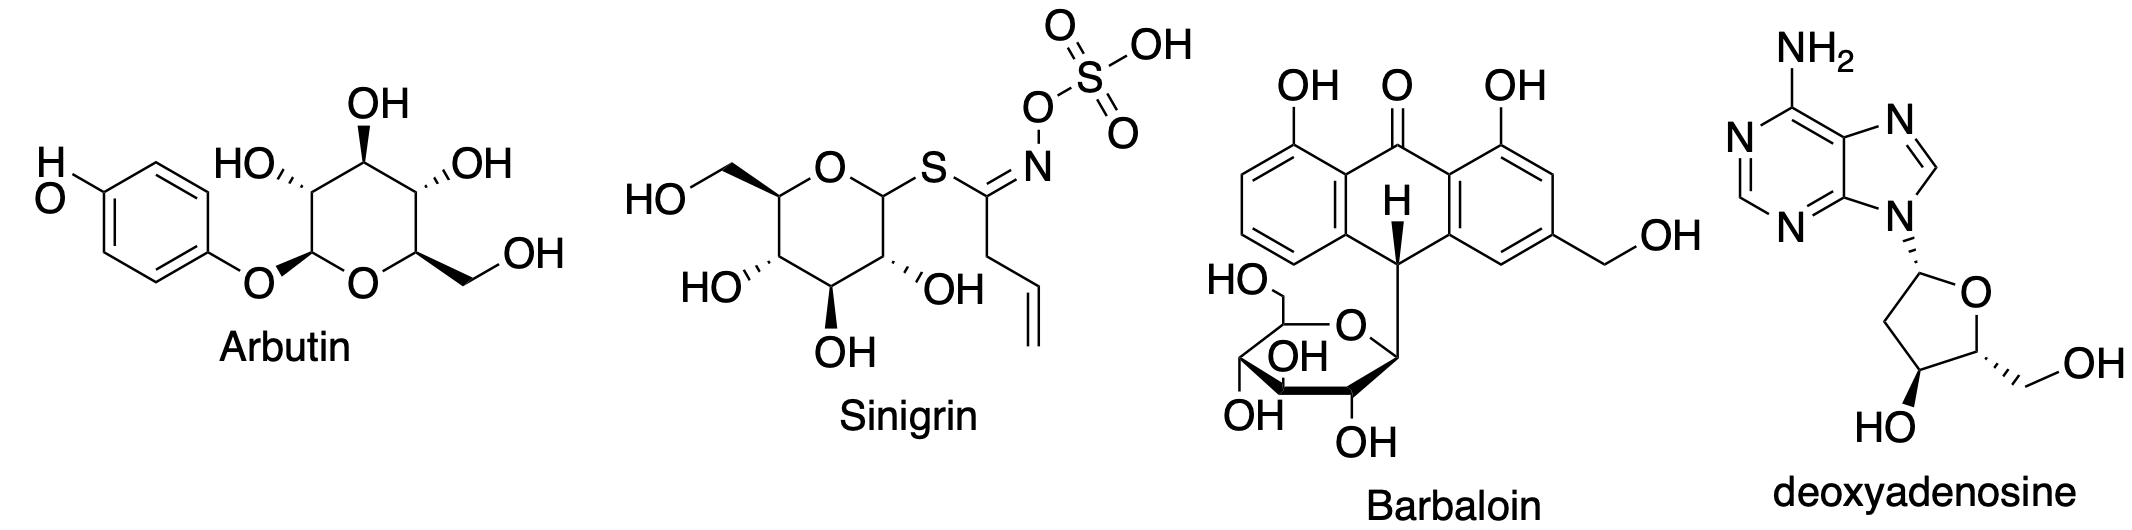
\includegraphics[width=\textwidth]{glycoside.png}
		\end{figure}
		\item Dựa vào Aglycone
	\end{itemize}
\end{frame}

\begin{frame}{Các chủ đề}
	\begin{columns}
		% Column 1
		\begin{column}{0.5\textwidth}
			\begin{itemize}
				\item Đại cương về Dược liệu 
				\item Nhóm Carbohydrate
				\item Nhóm Glycosid tim
				\item Nhóm Saponin 
				\item {\bf Nhóm Flavonoid}
			\end{itemize}
		\end{column}
		% Column 2
		\begin{column}{0.5\textwidth}
			\begin{itemize}
				\item Nhóm Alkaloid
				\item Nhóm Coumarin 
				\item Nhóm Anthranoid 
				\item Tinh dầu 
				\item Tanin 
			\end{itemize}
		\end{column}
		\end{columns}
\end{frame}

\begin{frame}{Mục tiêu học tập}
\begin{enumerate}
\item Khái niệm về cấu trúc hóa học của Flavonoid
\item Phân loại được các nhóm Flavonoid
\item So sánh được công thức cấu tạo Flavonoid
\item Lựa chọn phương pháp chiết xuất Flavonoid dựa vào tính chất lý hóa.
\item Tác dụng sinh học và chỉ định của Flavonoid
\end{enumerate}
\end{frame}
\begin{frame}{Tài liệu tham khảo}
	\begin{enumerate}
		\item Dược điển Việt Nam V
		\item Bài giảng Dược liệu, Đại học Dược Hà nội
		\item Medicinal Natural Products: A Biosynthesis Approach
		\item CARBON-13 NMR OF FLAVONOIDS
		\item TEXTBOOK OF PHARMACOGNOSY AND PHYTOCHEMISTRY
		\item Fundamentals of Pharmacognosy and phytotherapy
		\item https://www.ipni.org (Tra mã dược liệu- tên loài, tên họ)
		\item https://lotus.naturalproducts.net
		\item pubchem
	\end{enumerate}
\end{frame}
\section{Đại cương về Flavonoid}
\mysectionpage
\begin{frame}{Flavonoid Glycoside}
\tikzstyle{every node}=[anchor=west]
\tikzstyle{selected}=[draw=red,fill=red!30]
\tikzstyle{optional}=[dashed,fill=gray!50]
\begin{tikzpicture}[%
  grow via three points={one child at (0.5,-0.7) and
  two children at (0.5,-0.7) and (0.5,-1.4)},
  edge from parent path={(\tikzparentnode.south) |- (\tikzchildnode.west)}]
  \node {Glycoside}
    child { node {Anthraquinone Glycosides}}		
    child { node {Saponin Glycosides}}
    child { node {Steroid and Triterpenoid Glycosides}}
    child { node [selected] {Flavonoid Glycosides}
      child { node {O-glycoside}}
      child { node {C-glycoside}}
    }
    child [missing] {}				
    child [missing] {}						
    child { node {Cardiac Glycosides}}
	child { node {Coumarin Glycosides}}
	child { node {Cynophoric Glycoside}};
\end{tikzpicture}
\end{frame}
\begin{frame}{Phân loại tại Việt Nam}
	\begin{figure}
		\centering
		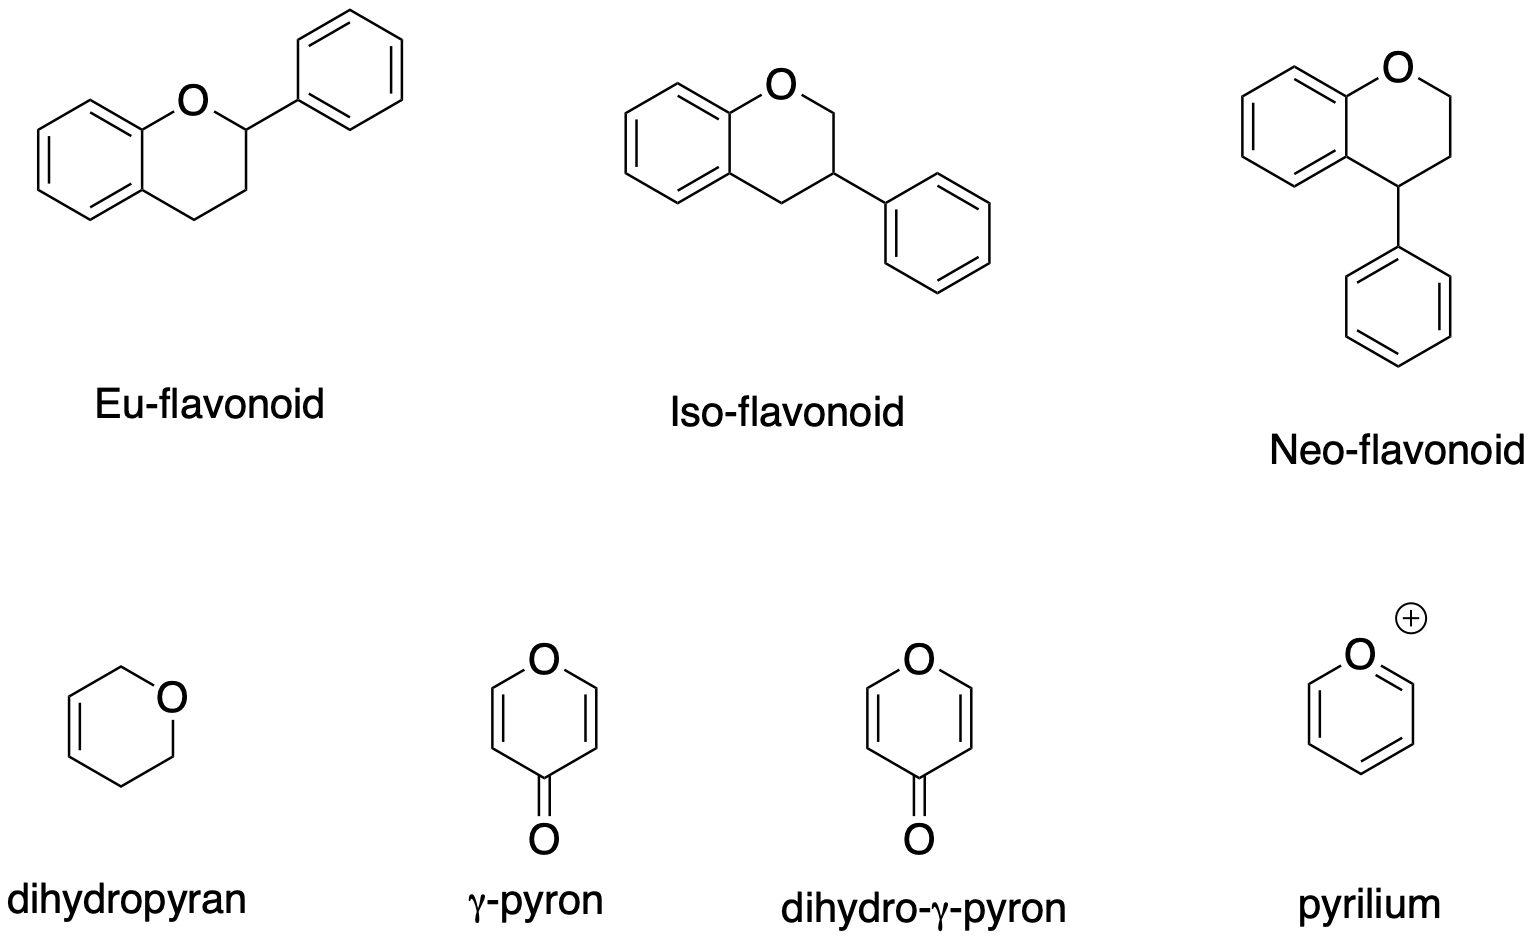
\includegraphics[scale=0.8]{Phan loai flavonoid o Viet nam.png}
	\end{figure}
	
\end{frame}
\begin{frame}{Aglycone of Flavonoid}
	\begin{figure}
		\centering
		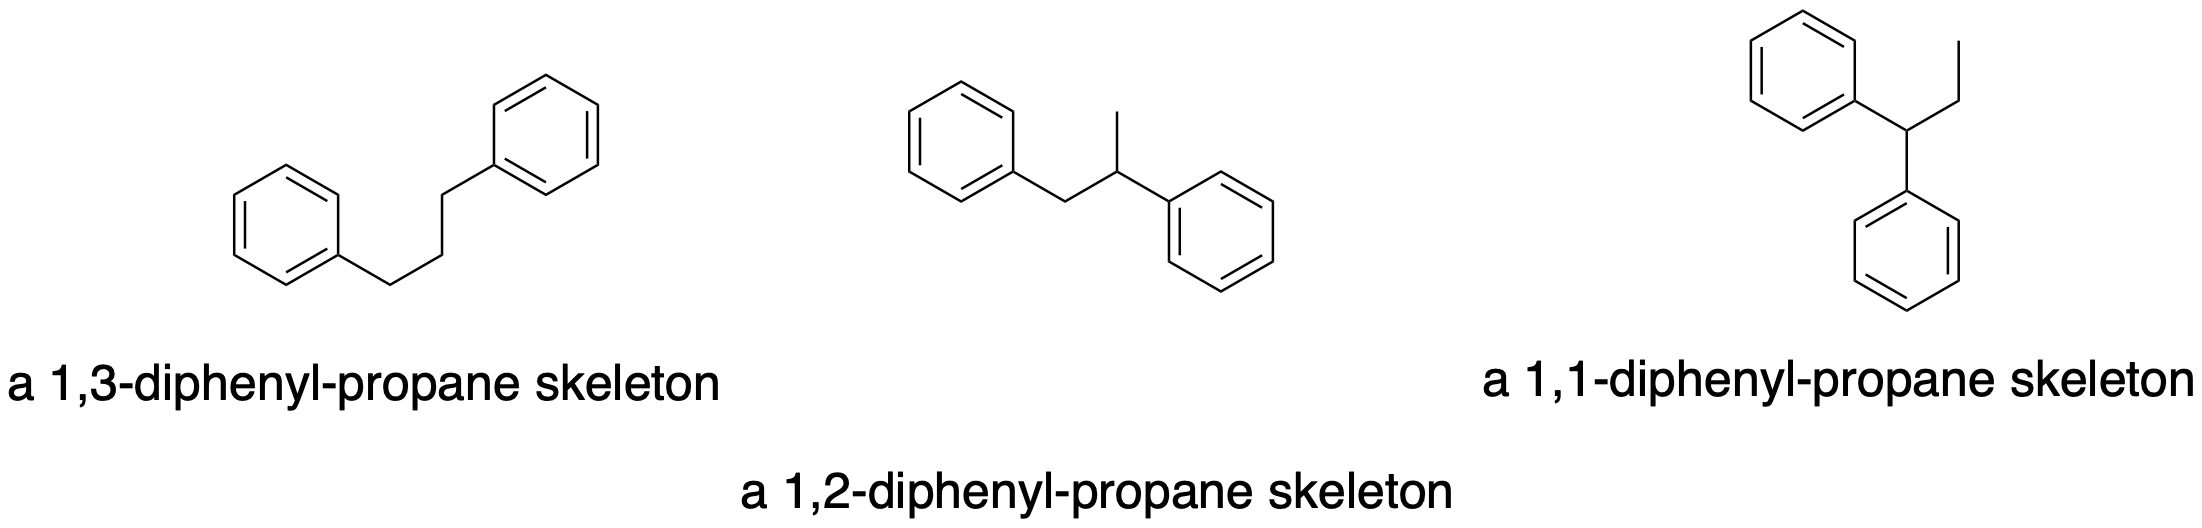
\includegraphics[scale=0.7]{Flavonoid skeleton.png}
	\end{figure}
\end{frame}

\begin{frame}{1,3-diphenyl-propane}
	\begin{figure}
		\centering
		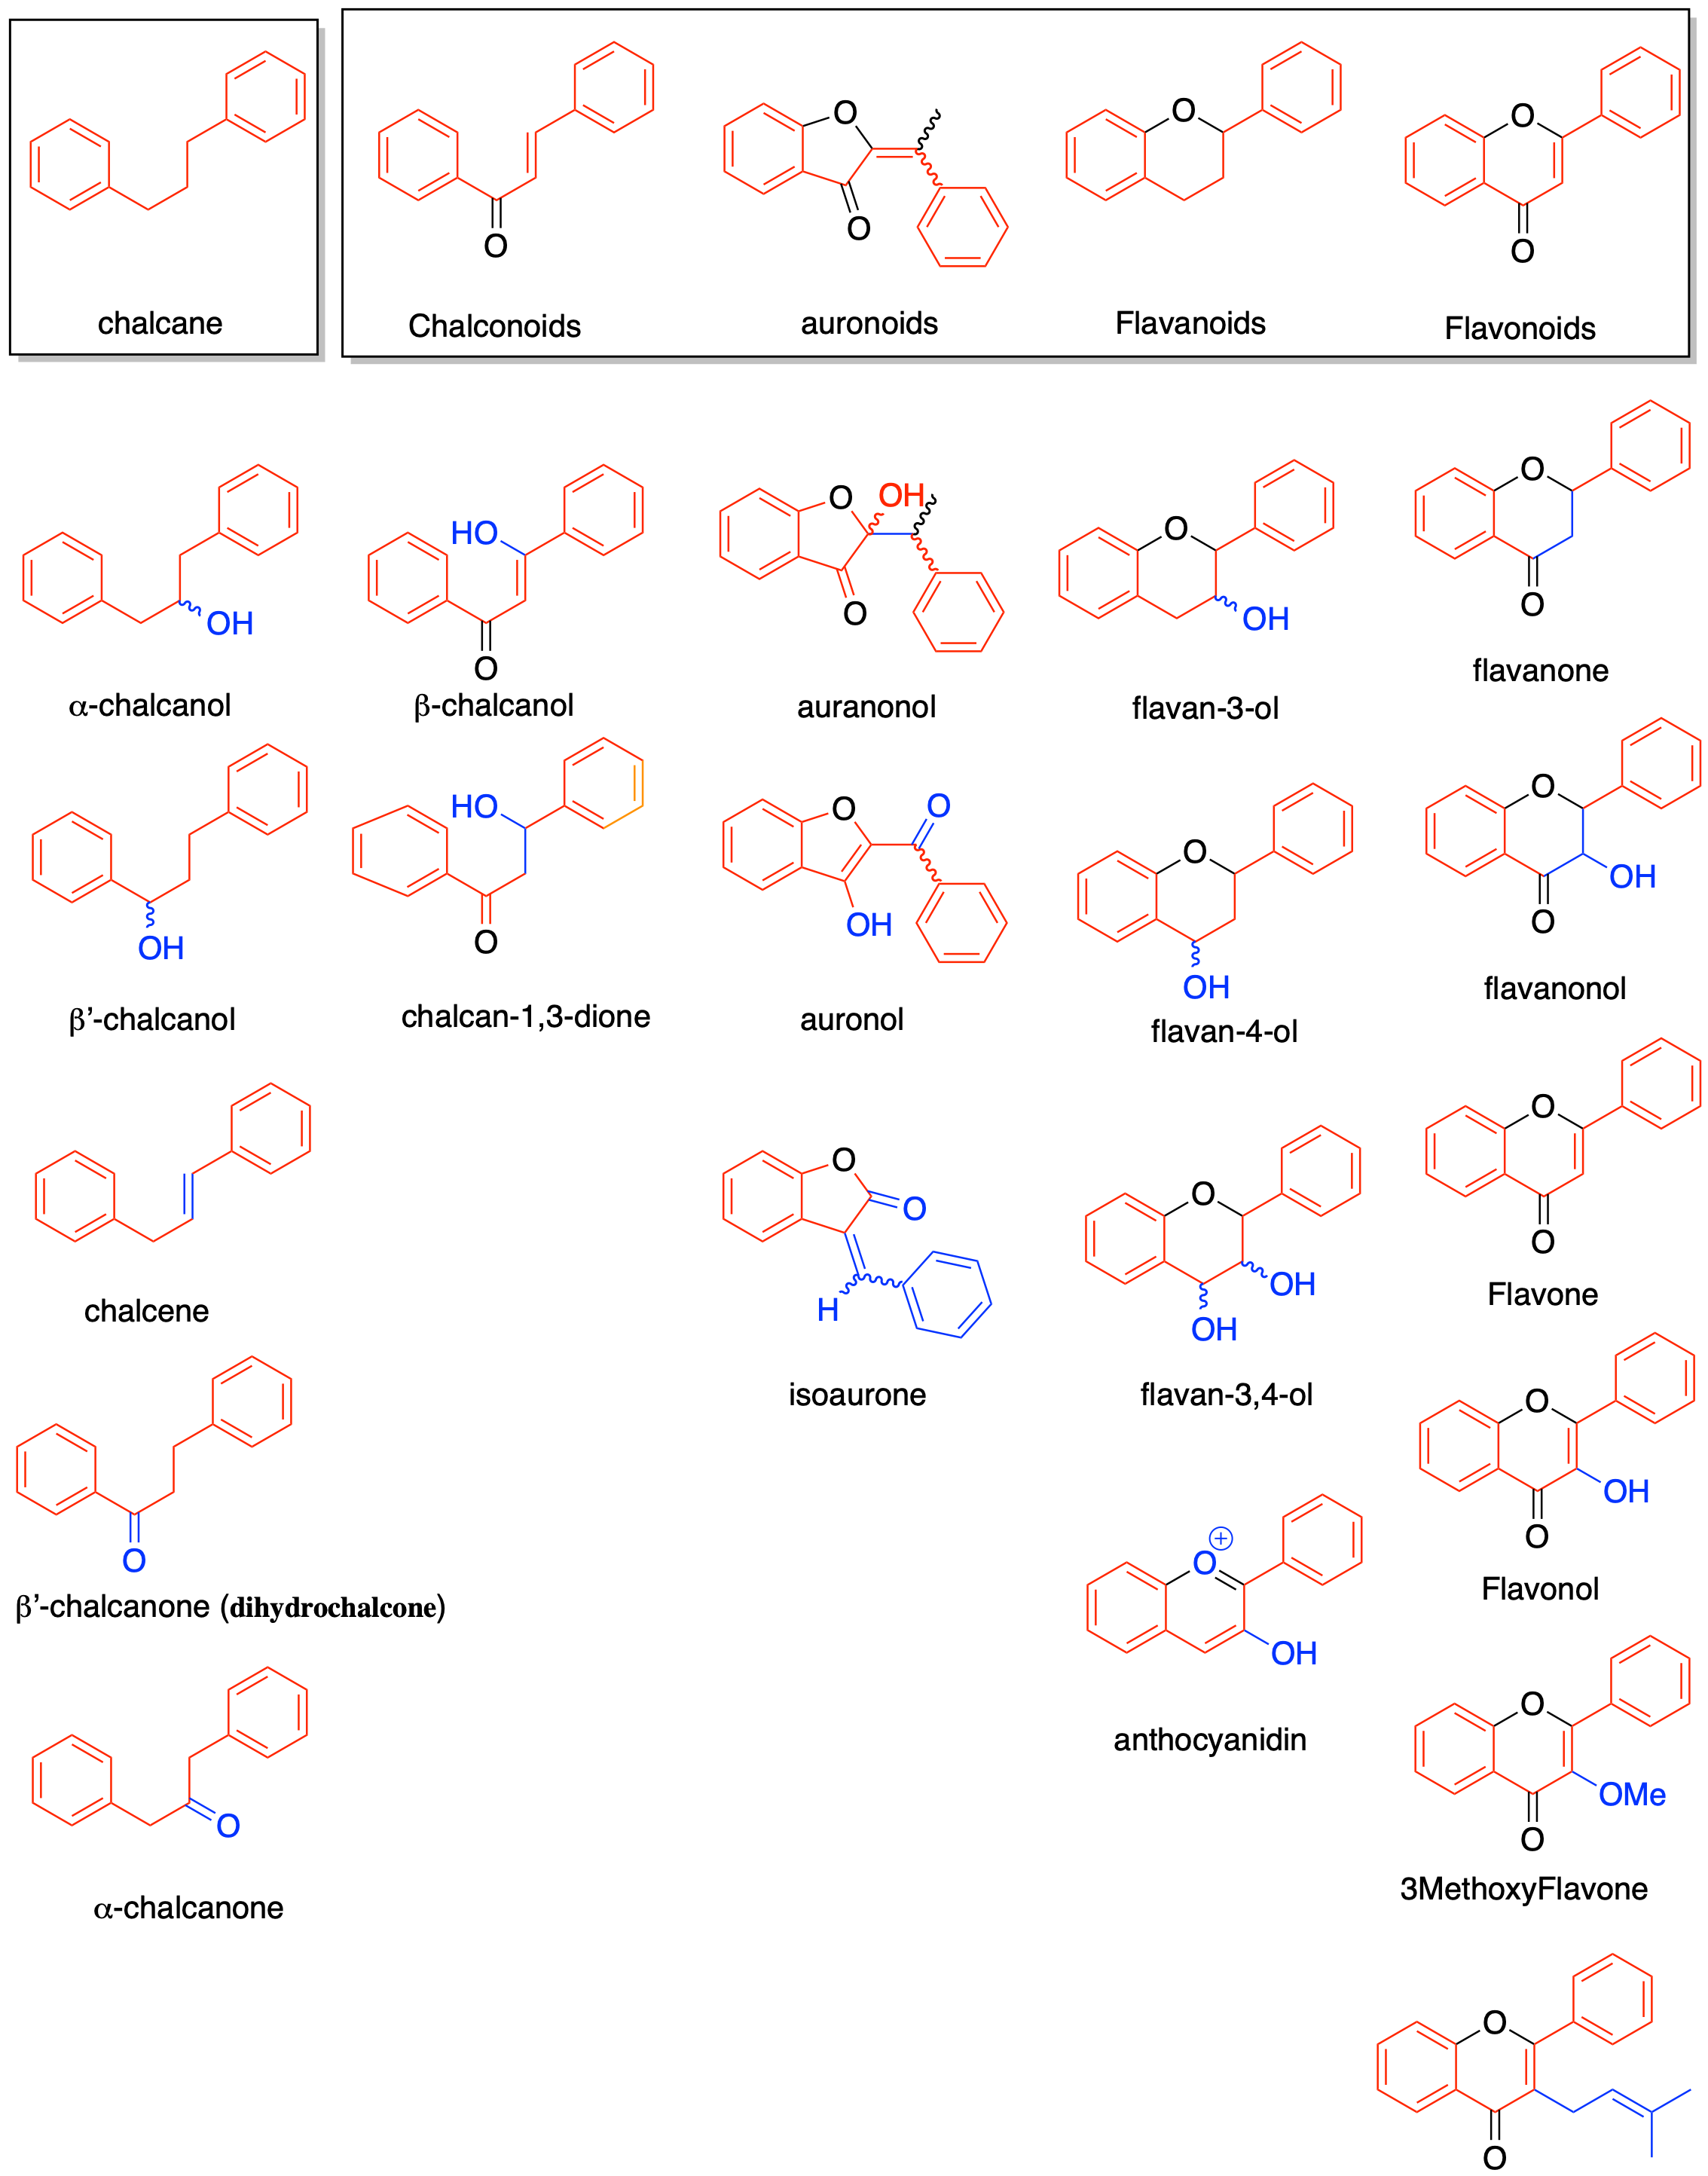
\includegraphics[height=0.8\textheight]{a 1,3-diphenyl-propane skeleton.png}
	\end{figure}
\end{frame}
\begin{frame}{1,2-diphenyl-propane}
	\begin{figure}
		\centering
		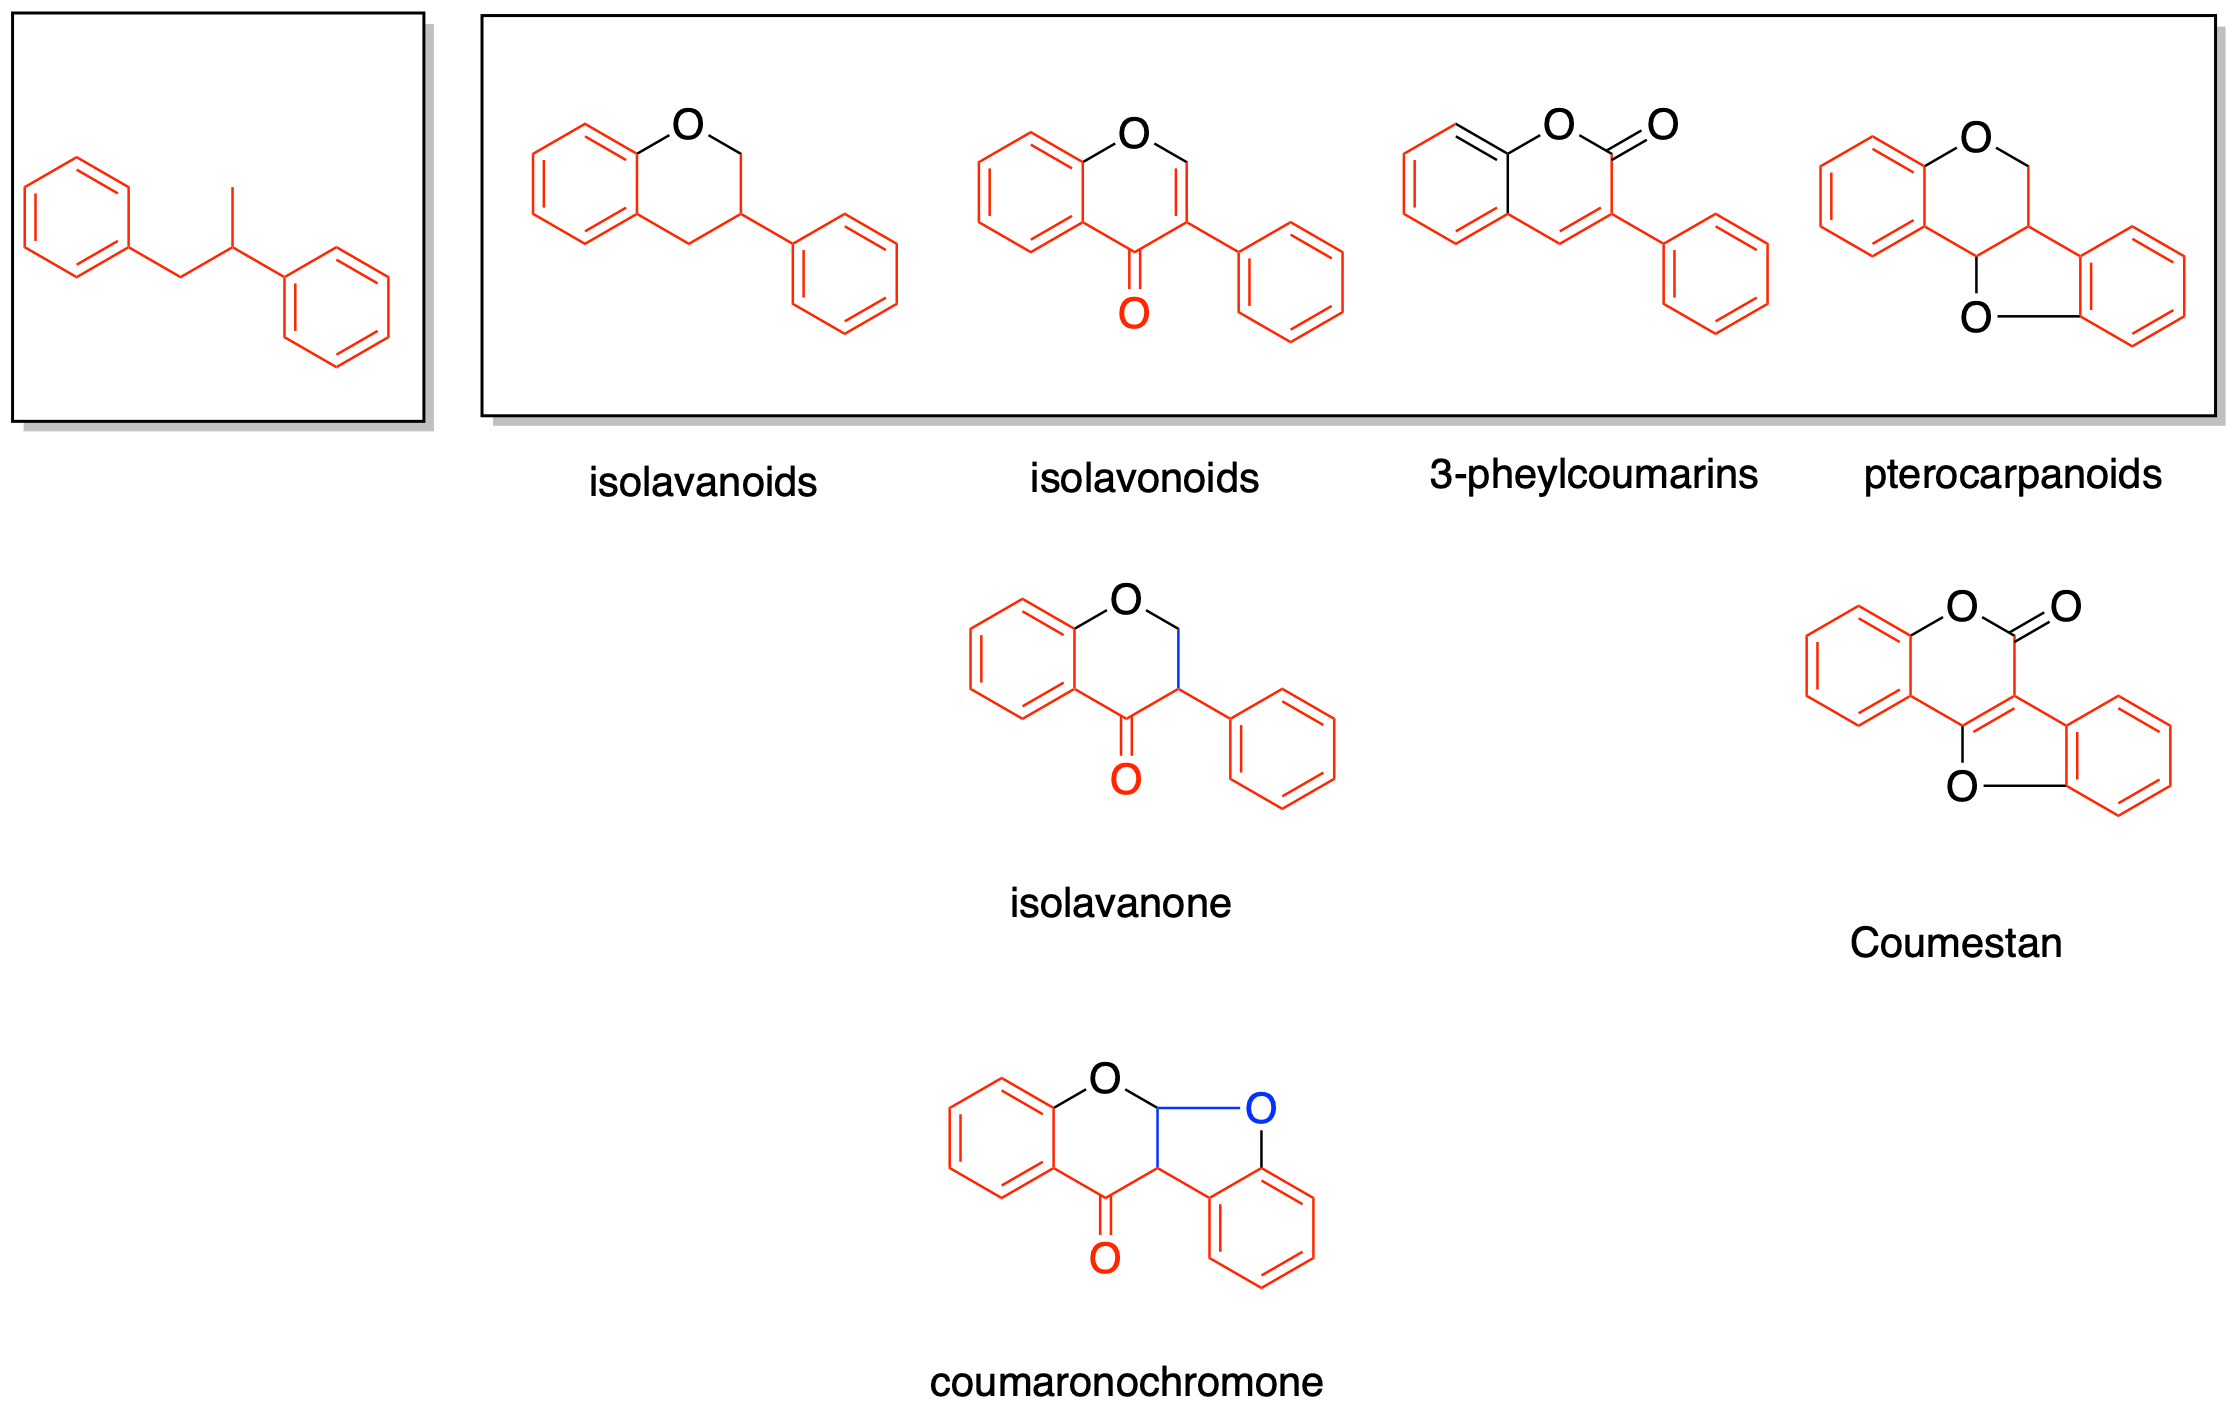
\includegraphics[scale=0.5]{1,2-diphenylpropane skeleton.png}
	\end{figure}
\end{frame}
\begin{frame}{1,1-diphenylpropane}
	\begin{figure}
		\centering
		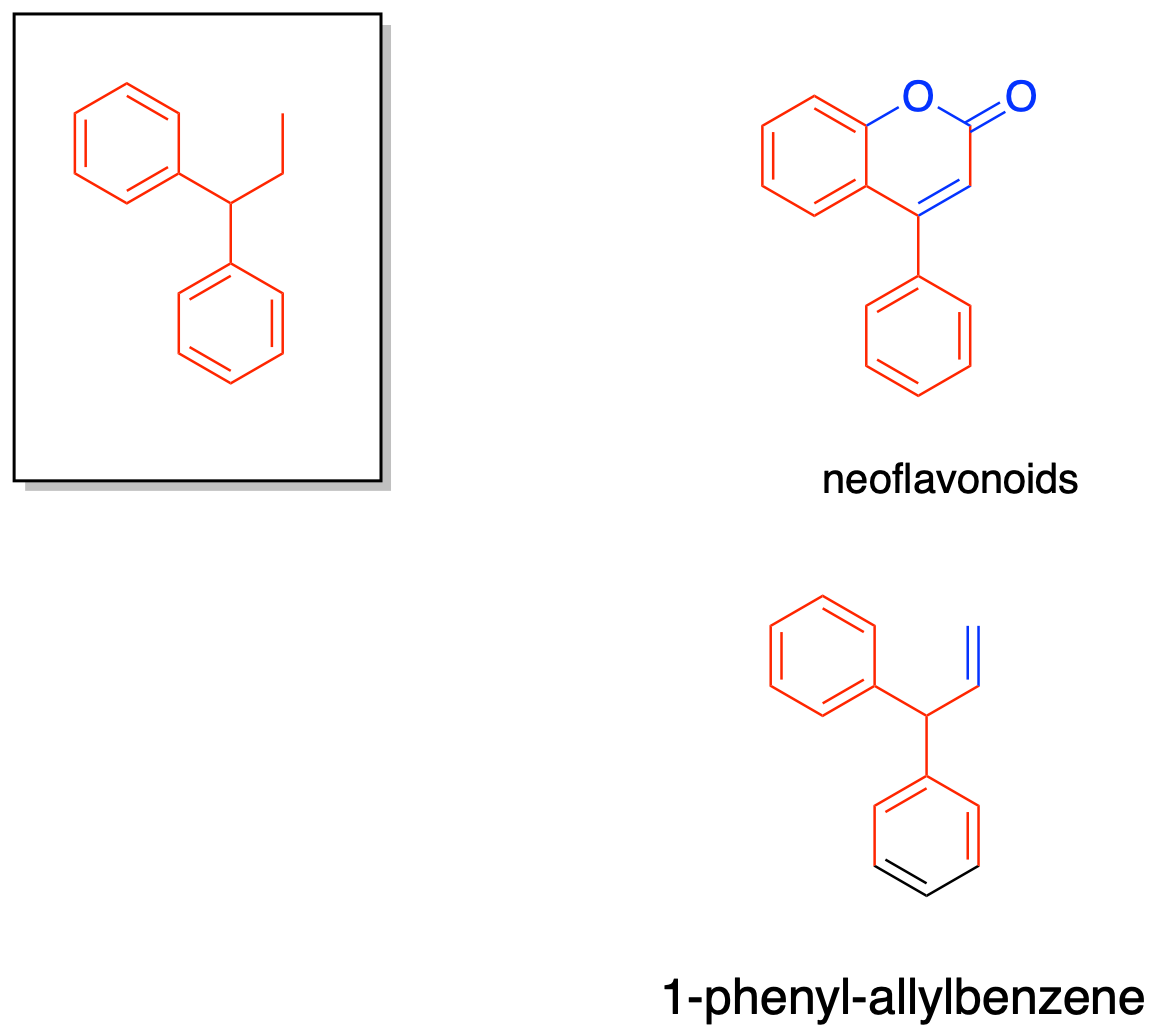
\includegraphics[scale=0.5]{1,1-diphenylpropane skeleton.png}
	\end{figure}
\end{frame}
\begin{frame}{Homoflavonoids}
	\begin{figure}
		\centering
		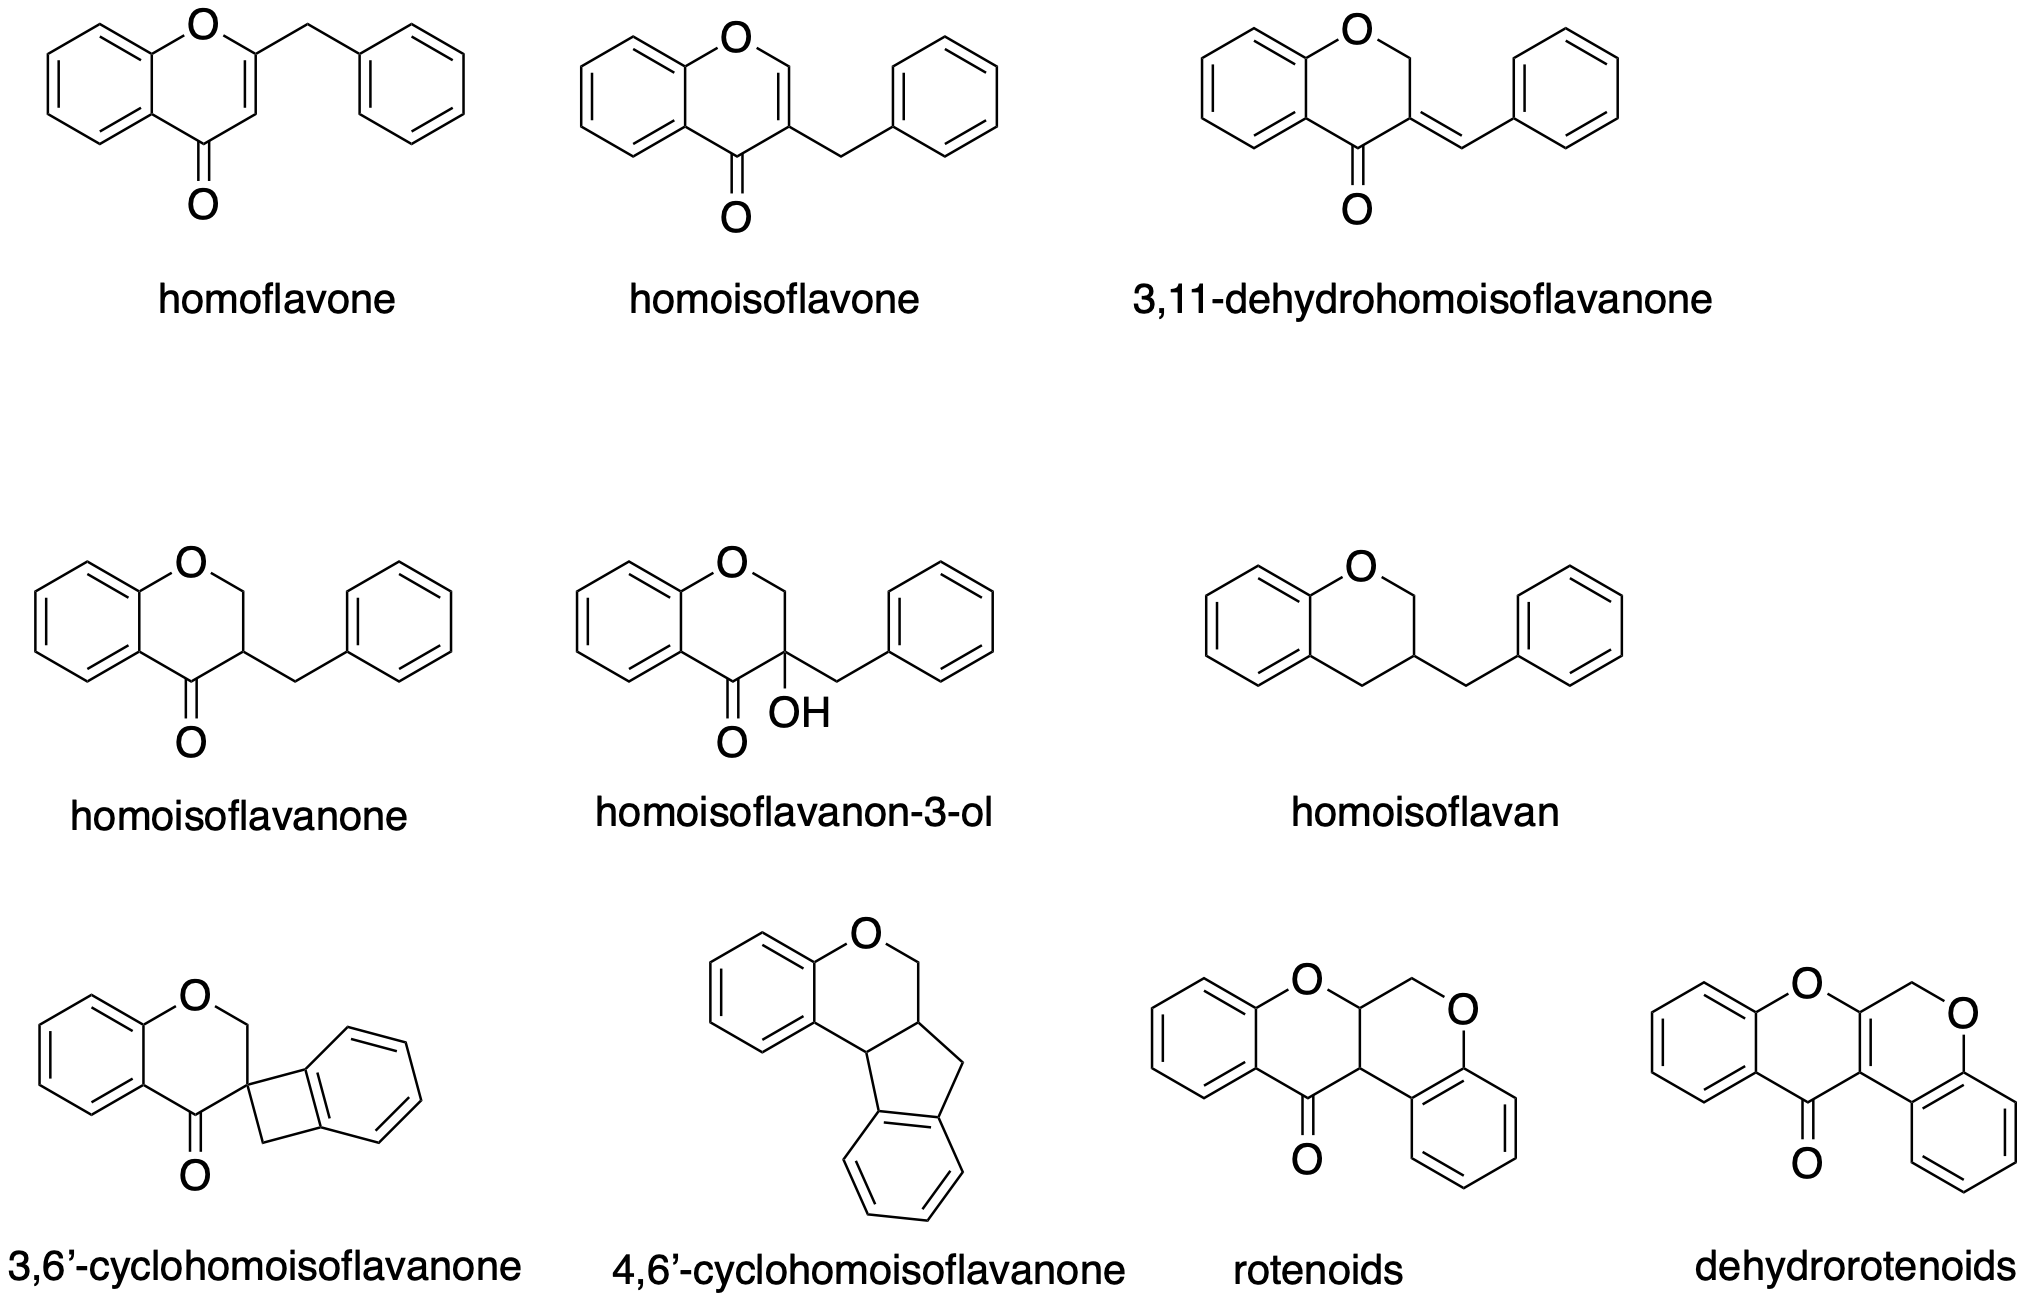
\includegraphics[scale=0.5]{homoflavonoids.png}
	\end{figure}
\end{frame}
\begin{frame}{Biosynthesis}

	\begin{figure}
		\centering
		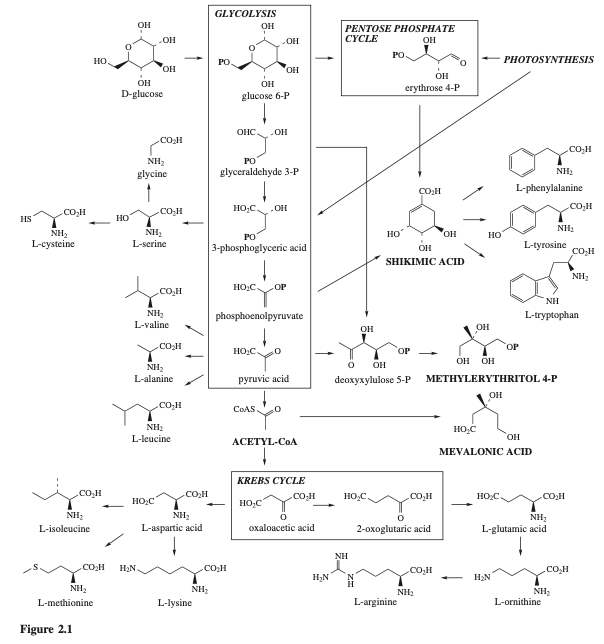
\includegraphics[scale=0.3]{Figure 2.1.png}
	\end{figure}
\end{frame}
\begin{frame}{THE SHIKIMATE PATHWAY}
	\begin{figure}
		\centering
		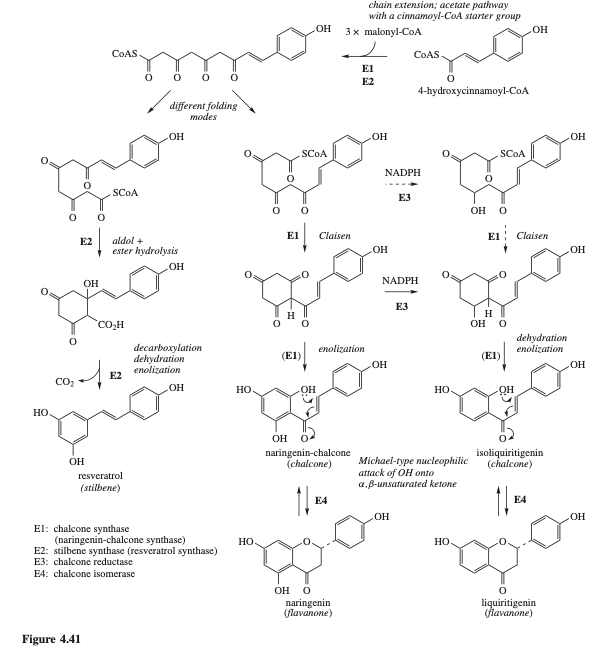
\includegraphics[scale=0.3]{Figure 4.41.png}
	\end{figure}
\end{frame}
\begin{frame}{THE SHIKIMATE PATHWAY}
	\begin{figure}
		\centering
		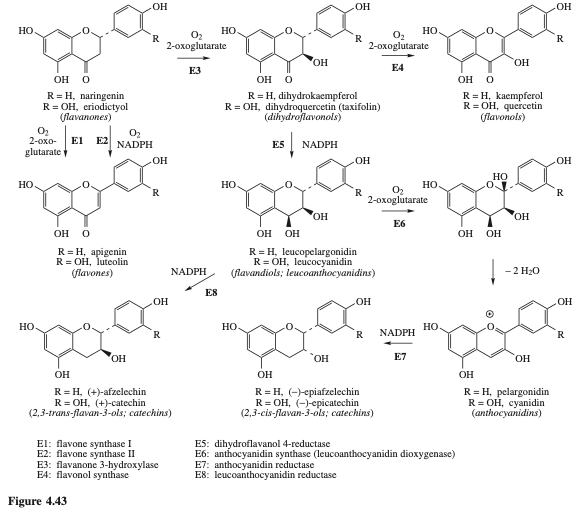
\includegraphics[scale=0.3]{Figure 4.43.png}
	\end{figure}
\end{frame}
\section{Phân bố Flavonoid}
\mysectionpage
\begin{frame}{Polyommatus icarus}
	\begin{figure}
		\centering
		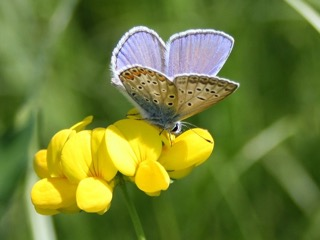
\includegraphics[scale=0.6]{Polyommatus.jpg}
		\caption{Loài bướm {\it Polyommatus icarus} 
		và hoa {\it Lotus corniculatus}}
	\end{figure}

\end{frame}
\begin{frame}{Phân bố trong thực vật}
\begin{columns}[T]
	\column{0.5\textwidth}
	\begin{figure}
		\centering
		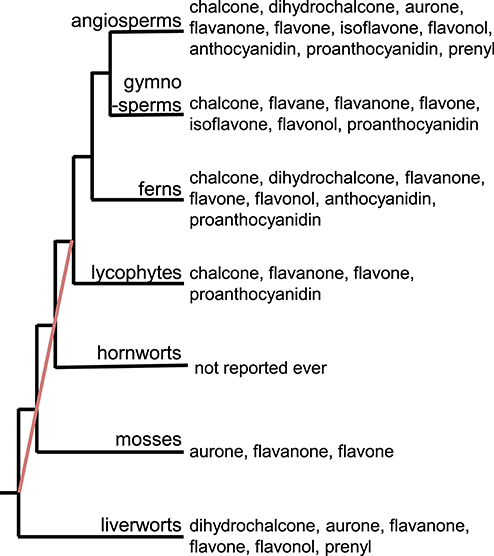
\includegraphics[scale=0.33]{Flavonoid distribution.jpg}
	\end{figure}
	\column{0.5\textwidth}
	{\footnotesize
	\begin{itemize}
		\item Thực vật hạt kín (Angiosperms)
		\item Thực vật hạt trần (Gymnospermae)
		\item Ngành dương sỉ (Ferns)
		\item Ngành thạch tùng (Lycophytes)
		\item Ngành rêu sừng (Hornworts)
		\item Ngành rêu (Mosses)
		\item Ngành rêu tản (Liverworts)
	\end{itemize}
	}
\end{columns}
\end{frame}

\begin{frame}
	\begin{columns}[T]
		\column{0.3\textwidth}
		\begin{figure}
			\centering
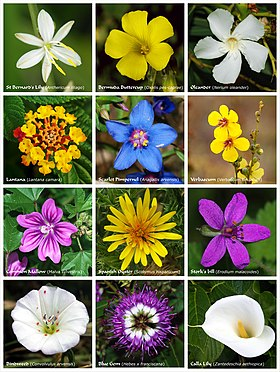
\includegraphics[height=0.35\textheight, width=\textwidth]{angiosperms.jpg}
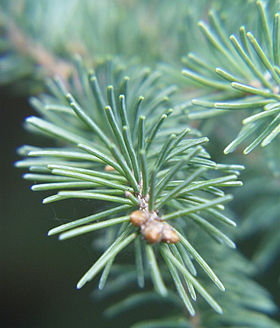
\includegraphics[height=0.35\textheight, width=\textwidth]{gymnospermae.jpg}
		\end{figure}
		\column{0.3\textwidth}
		\begin{figure}
			\centering
			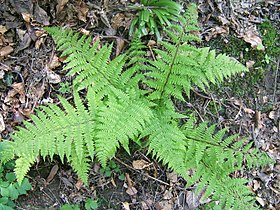
\includegraphics[height=0.35\textheight, width=\textwidth]{Ferns.jpg}
			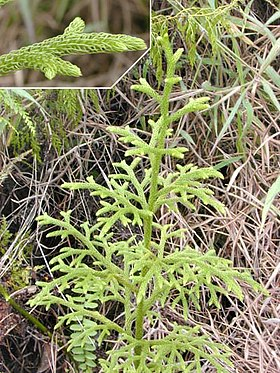
\includegraphics[height=0.35\textheight, width=\textwidth]{Lycopodium_plant.jpg}
		\end{figure}
		\column{0.3\textwidth}
		\begin{figure}
			\centering
			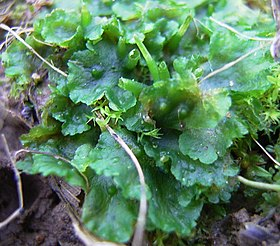
\includegraphics[height=0.25\textheight, width=\textwidth]{Phaeoceros_laevis.jpg}
			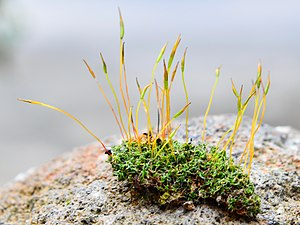
\includegraphics[height=0.25\textheight, width=\textwidth]{Moss_Gametophytes_Sporophytes.JPG}
			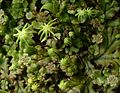
\includegraphics[height=0.25\textheight, width=\textwidth]{Marchantia.jpg}
		\end{figure}
	\end{columns}
\end{frame}


\section{Tính chất Hóa lý}
\mysectionpage
\begin{frame}{Đặc tính hóa lý $\rhd$ Màu sắc}
	\begin{itemize}
		\item Flavon: Vàng rất nhạt có khi không màu 
		\item Flavonol: Vàng nhạt đến vàng
		\item Chalcon và auron: Vàng đậm đến đỏ cam
		\item Các chất thuộc nhóm isoflavon, flavanon, isoflavanon, flavanonol, leuco-anthocyanidin, flavan-3-ol: Không màu
		\item Anthocyanidin: Màu thay đổi theo pH môi trường(màu đỏ trong môi trường acid, màu xanh trong môi trường base)
	\end{itemize}
Flavonoid ở trong các bộ phận của cây thì còn phụ thuộc vào hỗn hợp với các sắc tố khác 
\end{frame}
\begin{frame}{Đặc tính hóa lý$\rhd$Độ tan}
	\begin{itemize}
		\item Dạng Glucoside: dễ tan trong nước và dung môi phân cực
		\item Dạng Aglycone: Tan trong dung môi hữu cơ, khó tan trong nước
	\end{itemize}
\end{frame}
\begin{frame}{INFRA-RED SPECTROSCOPY}
	The IR spectra of all the flavonoids and isoflavonoids show absorption
 bands in the region 1500-1600 $cm^{-1}$ due to aromatic rings, along with a carbonyl band at 1620-1670 $cm^{-1}$ . The carbonyl absorption does not appear in flavanoids, isoflavanoids pterocarpanoids and chalcanoids. The presence of hydroxyl groups in hydroxyflavonoids is evidenced by absorption in
the region 3300-3450 $cm^{-1}$ . An absorption at  925 $cm^{-1}$ is indicative of a methylenecioxy group and the presence of a gem-dimethyl group is indicated by the appearance of a band at 1400 $cm^-1$ . The glycosidic nature of a flavonoid is reflected by broad bands at  3250 and 1060 $cm^{-1}$. However, although these absorption bands are present in most flavonoid glycoside.
\end{frame}
\begin{frame}{UV-Vis SPECTROSCOPY}
	\begin{figure}
		\centering
		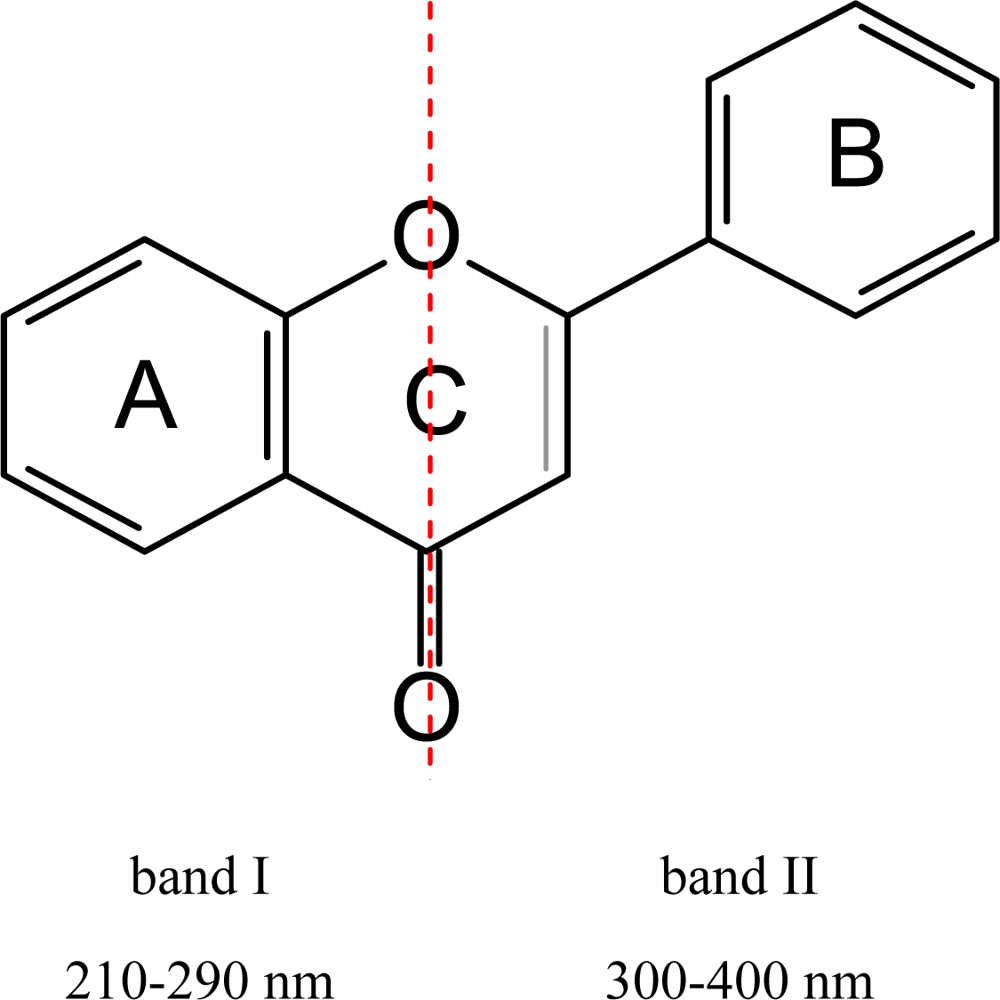
\includegraphics[scale=0.2]{ijms-11-00595f10}
	\end{figure}
\end{frame}

\begin{frame}{UV-Vis SPECTROSCOPY}

	% Please add the following required packages to your document preamble:
% \usepackage{graphicx}
\begin{table}[]
	\resizebox{\textwidth}{!}{%
	\begin{tabular}{lll}
	\hline
	\textbf{Band II}                                                  & \textbf{Band I}  & \textbf{Flavonoid type}                 \\ \hline
	250-280                                                           & 304-350          & Flavones                                \\
	250-280                                                           & 328-360          & Flavonols (3-OH substituted)            \\
	250-280                                                           & 350-385          & Flavonols (3-OH free)                   \\
	245-275                                                           & 310-330 Shoulder & Isoflavones                             \\
	245-275                                                           & 320 peak         & Isoflavones (5-deoxy, 6,7-dioxygenated) \\
	\begin{tabular}[c]{@{}l@{}}230-270\\ (low intensity)\end{tabular} & 340-390          & Chalcones                               \\
	\begin{tabular}[c]{@{}l@{}}230-270\\ (low intensity)\end{tabular} & 380-430          & Aurones                                 \\
	270-280                                                           & 465-560          & Anthocyanidins and anthocyanins         \\ \hline
	\end{tabular}%
	}
	\end{table}
\end{frame}
\begin{frame}{Luteolin and derivatives$\rhd$UV spectrum}
	\begin{figure}
		\centering
		\includegraphics[scale=0.3]{luteolin 1 and derivatives .png}
	\end{figure}
\end{frame}
\begin{frame}{Anthocyanidins}{Int. J. Mol. Sci. 2010, 11(2), 595-621}
	\begin{figure}
		\centering
		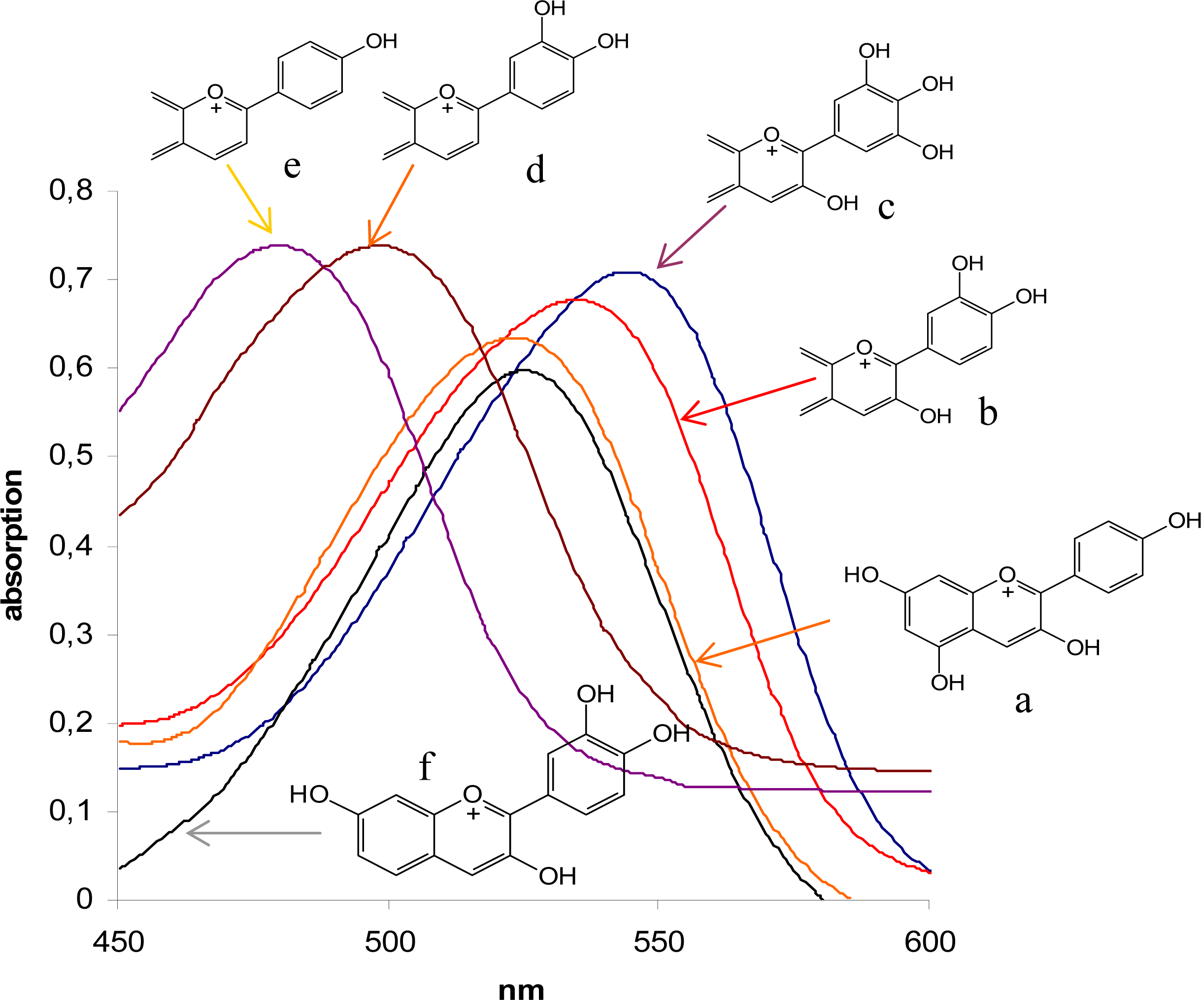
\includegraphics[scale=0.2]{ijms-11-00595f11.png}
	\end{figure}
\end{frame}
\begin{frame}{Anthocyanidins$\rhd$Int. J. Mol. Sci. 2010, 11(2), 595-621}
	\begin{figure}
		\centering
		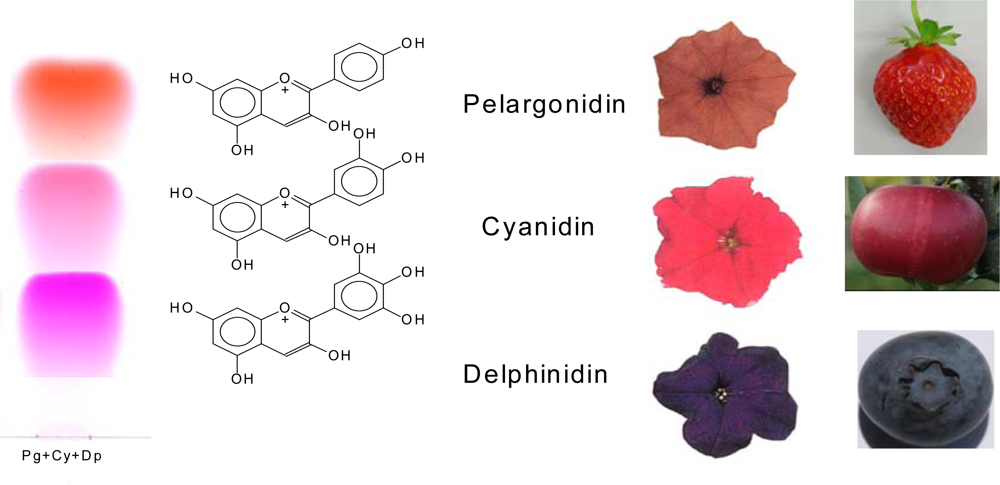
\includegraphics[scale=0.3]{ijms-11-00595f13.png}
	\end{figure}
\end{frame}
\section{Định tính và định lượng}
\mysectionpage
\begin{frame}{Định tính bằng phản ứng hóa học}
\begin{enumerate}
	\item Phản ứng Cyanidin (Shinoda): Tác dụng với tác nhân khử như hydro, vòng $\gamma $- pyron bị khử thành nhân pyrilium có màu đỏ tươi 
	\item Phản ứng với kim loại nặng:
	\begin{itemize}
		\item Với muối $Fe^{3+}$ tạo phức màu đen, xanh tím 
		\item Với muối $Al^{3+}$ tạo phức màu vàng
	\end{itemize}
	\item Phảm ứng với kiễm loãng
	\item Phản ứng với muối diazoni 
	\item Các phản ứng khác
\end{enumerate}
\end{frame}
\begin{frame}{Phản ứng tạo màu Cyanidin (Shinoda)}
	\begin{figure}
		\centering
		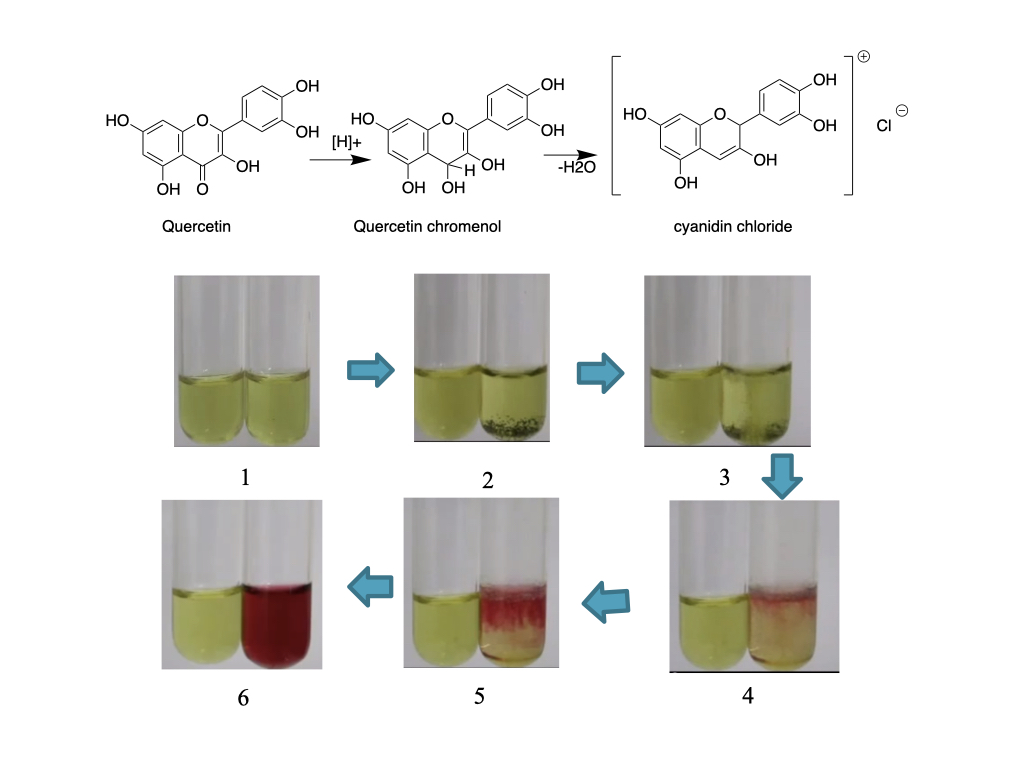
\includegraphics[scale=0.25]{Phan ung Cyanidine.jpeg}
	\end{figure}
\end{frame}
\begin{frame}{Tạo màu với $Fe^{3+}$}
	\begin{figure}
		\centering
		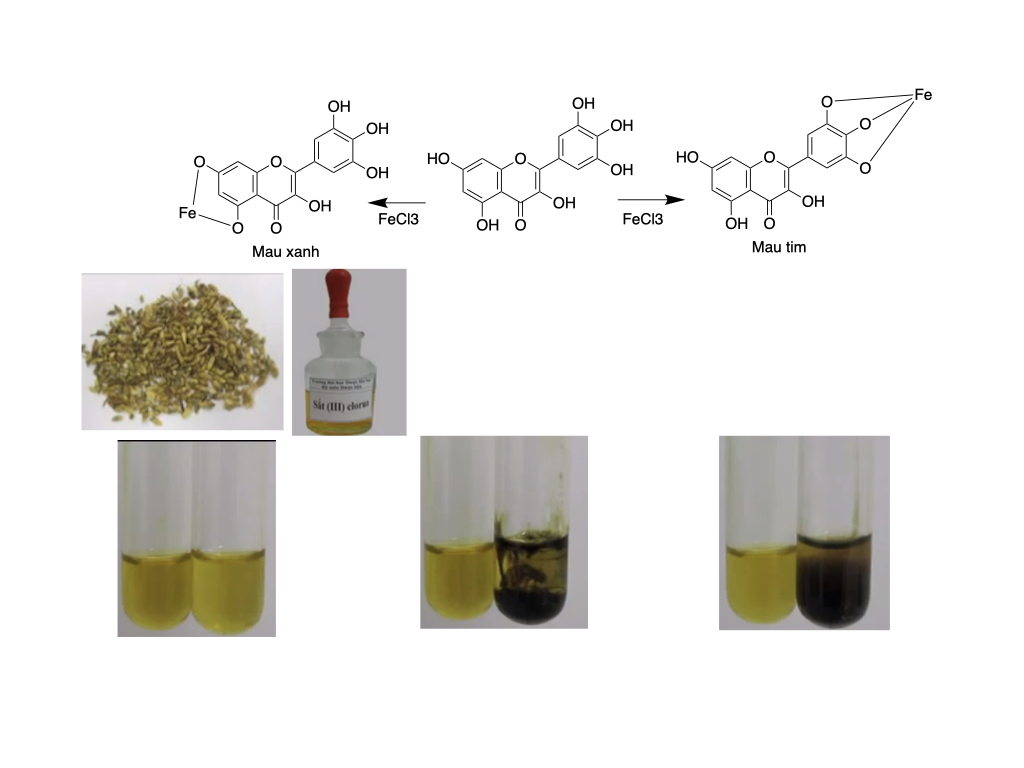
\includegraphics[scale=0.25]{Phan ung Fe.jpeg}
	\end{figure}
\end{frame}
\begin{frame}{Các phản ứng khác}
	\begin{figure}
		\centering
		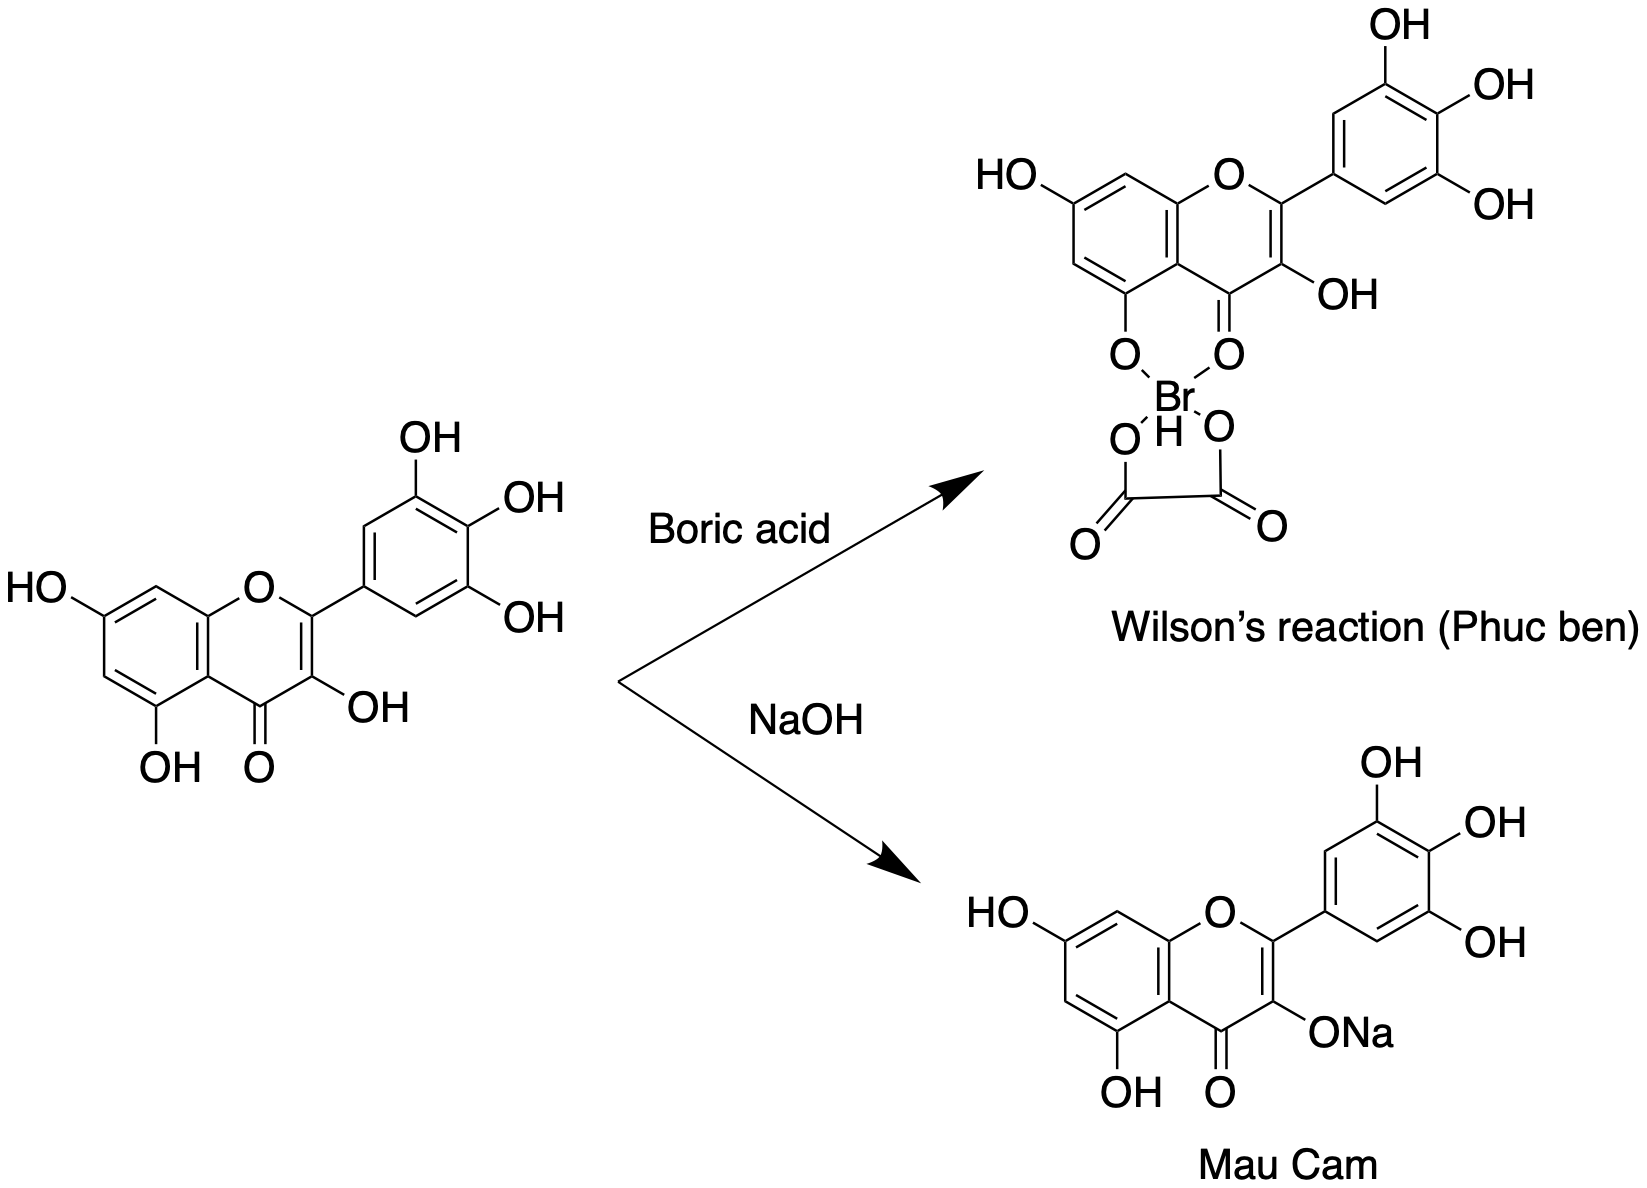
\includegraphics[scale=0.6]{Tao phan ung khac.png}
	\end{figure}
\end{frame}
\begin{frame}{Định tính bằng TLC}
	\begin{itemize}
		\item So với chất chuẩn
		\item So với dược liệu đối chiếu (???)
	\end{itemize}
\end{frame}
\begin{frame}{Phương pháp định tính Flavonoid}{Chromatographic Fingerprint Analysis of Herbal Medicines}
    \begin{itemize}
        \item Chiết bằng MeOH
        \item Silica gel/HPTLC Silica gel
        \item Ethyl acetate-Formic acid-Glacial acetic acid- Water (10 + 1.1 + 1.1 + 2.6)
        \item Thuốc thử hiện màu
    \end{itemize}
\end{frame}

\begin{frame}{Phương pháp định tính Flavonoid$\rhd$aluminium(III)chloride-reagent}
    \begin{figure}
        \centering
        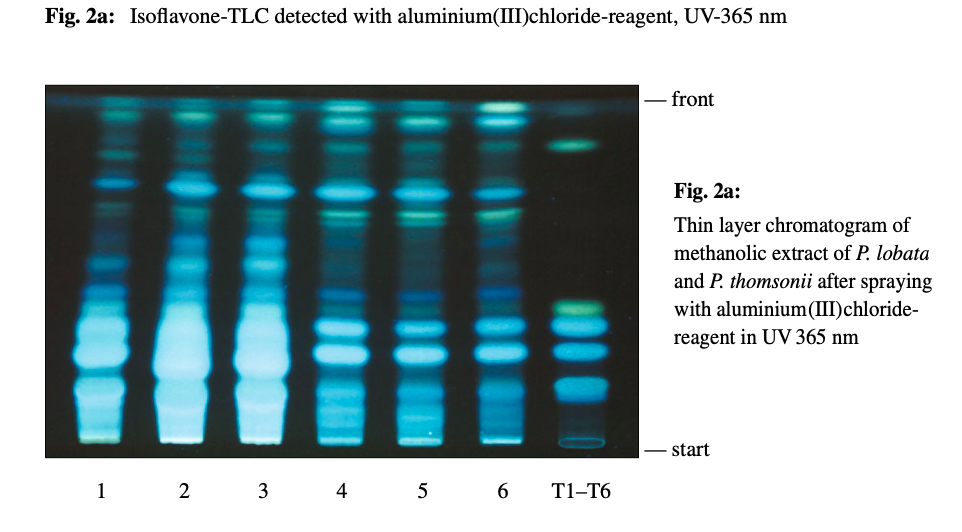
\includegraphics[width=0.8\textwidth]{P. lobata and P. thomsonii.png}
		\caption{5 \% AlCl3 x 6 H2O dissolved in ethanol 80 \%). The plate is intensively sprayed with 10 ml solution and then exposed to UV 366 nm for 30 minutes.}
    \end{figure}
\end{frame}

\begin{frame}{Phương pháp định tính Flavonoid$\rhd$fast blue salt-reagent}
    \begin{figure}
        \centering
        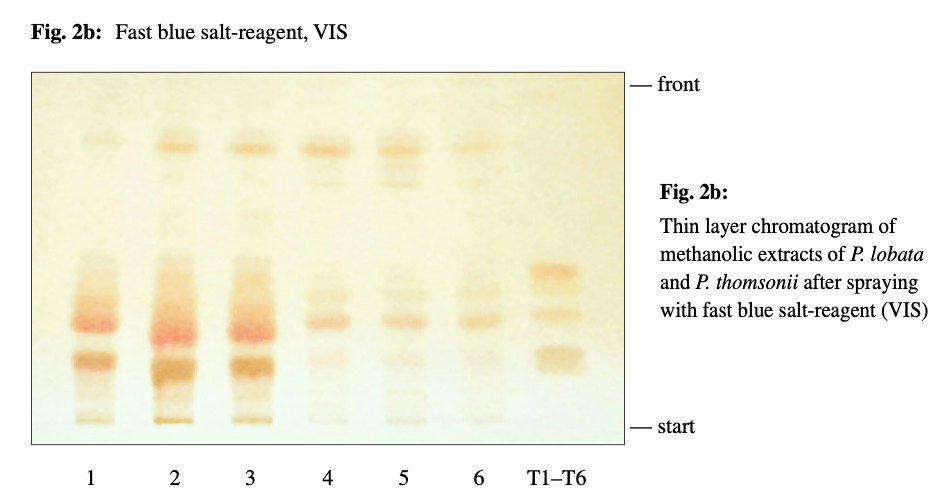
\includegraphics[width=0.8\textwidth]{Fast blue salt-reagent.png}
        \caption{\tiny{
        {\bf I:} 0.5 \% fast blue salt B = $3,3^\prime-dimethoxybiphenyl–4,4^\prime bis (diazonium)-dichloride$ is dissolved in methanol 80 \%.
        {\bf II:} 5 \% potassiumhydroxid in methanol 80 \%.
        The plate is intensively sprayed with 10 ml solution I and then immediately sprayed with 10 ml solution II. The evaluation is carried out in VIS.}}
    \end{figure}
	
\end{frame}

\begin{frame}{Phương pháp định tính Flavonoid$\rhd$Natural products-polyethylene glycol reagent (NP/PEG)}
    \begin{figure}
        \centering
        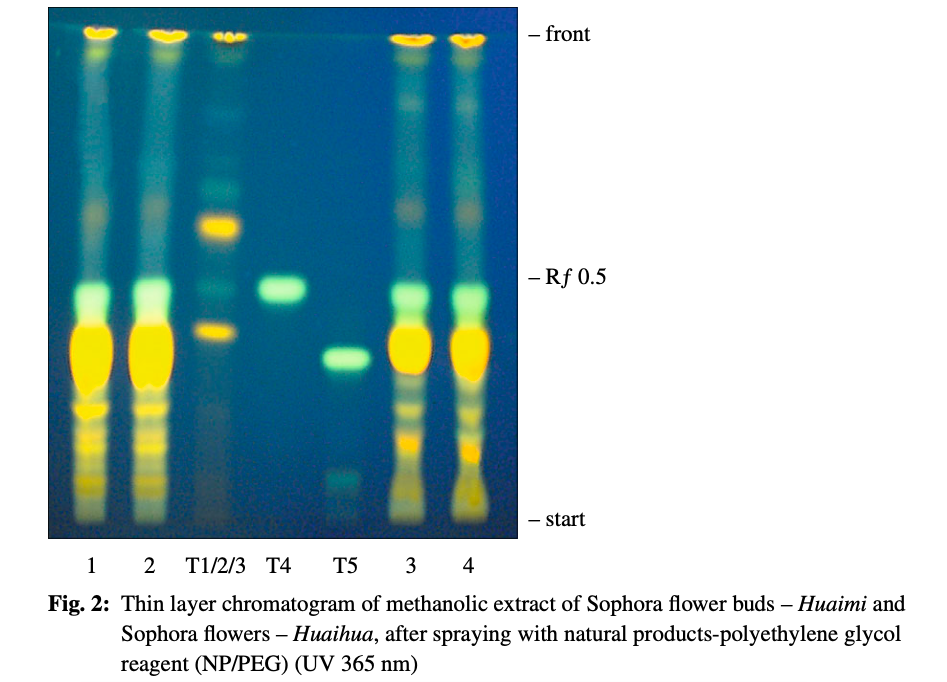
\includegraphics[width=0.6\textwidth]{Sophora flower buds Flavonoid.png}
        \caption{\tiny {\bf I:} 1 \% diphenylboric acid-$\beta$-ethylamino ester (=diphenylboryloxyethylamine, NP) in methanol. 
		{\bf II:} 5 \% polyethylene glycol-4000 (PEG) in ethanol.
        The plate is sprayed first with solution I and then with solution II.}
    \end{figure}
\end{frame}

\begin{frame}{Định tính bằng HPLC}{Fingerprint của Hòe Hoa}
\begin{figure}
	\centering
	
	\includegraphics[height=0.4\textheight]{Sophorae flos – Huaihua Fingeprint.png}
	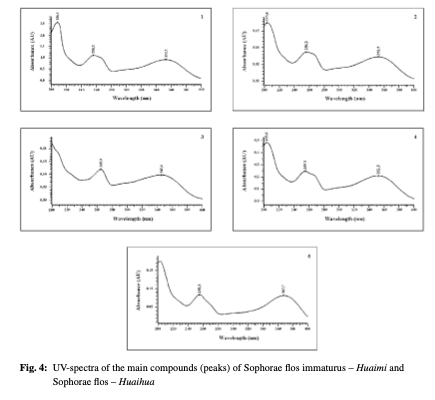
\includegraphics[height=0.4\textheight]{Sophora japonica-UV.png}
	\includegraphics[height=0.3\textheight]{Sophorae flos – Huaihua Retation time.png}
\end{figure}
	
\end{frame}
\begin{frame}{Định lượng}
	\begin{enumerate}
		\item Phương pháp cân 
		\item Phương pháp đo quang 
		\item Phương pháp HPLC
	\end{enumerate}
\end{frame}
\begin{frame}{Định lượng bằng phương pháp cân}
Ứng dụng đối với nguyên liệu giàu flavonoid và dịch chiết ít tạp chất, ví dụ.
\begin{itemize}
	\item Định lượng flavonoid trong thịt quả mơ ({\it Prunus armeniaca}) bằng phương pháp cân: Bột dược liệu chiết bằng CHCl3 trên bình Soxhlet để loại tạp, sấy khô. Chiết bằng EtOH 96\% trên bình Soxhlet thu lấy dịch, sau đó bốc hơi dung môi. Chiết lại bằng nước nóng sau đó chiết bằng EtOAc bay hơi dung môi. Thu được cắn. Cân cắn để xác định lượng flavonoid toàn phần. 
	\item Định lượng rutin trong nụ hoa hòe ({\it Sophora japonica}): loại tạp bằng HCl 0.5\%, chiết bằng EtOH 96\% nóng, thủy phân bằng $H_2SO_4$ , quercetin rất ít tan được lọc và cân rồi tính ra rutin.\\ 
\end{itemize}
Phương pháp này có ưu điểm là thực hiện nhanh, dễ thực hiện tuy nhiên sai số 
mắc phải lớn. \\
\end{frame}
\begin{frame}{Phương pháp đo quang UV-Vis\tiny{\it Petr Struchkov et al, 2018}}
	\begin{figure}
		\centering
		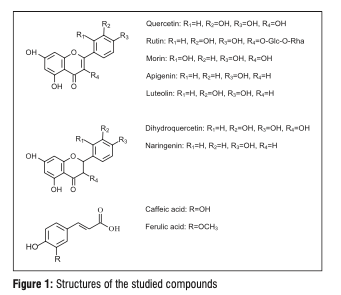
\includegraphics[scale=0.4]{Flavonoid UV.png}
	\end{figure}
	{\footnotesize
	\begin{itemize}
		\item Nitrozation
		\item Complex formation with aluminum chloride (Method 1)
		\item Nitrozation and complex formation with aluminum chloride (Method 2)
		\item Reaction with dinitrophenylhydrazine
	\end{itemize}
	}
\end{frame}
\begin{frame}{Phương pháp đo quang UV-Vis \tiny{ \it Petr Struchkov et al, 2018}}
	\begin{columns}[]
		\column{0.3\textwidth}
		\begin{figure}
			\centering
			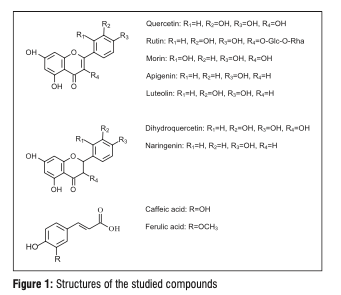
\includegraphics[width=\textwidth]{Flavonoid UV.png}
		\end{figure}
		\column{0.7\textwidth}
		\begin{figure}
			\centering
			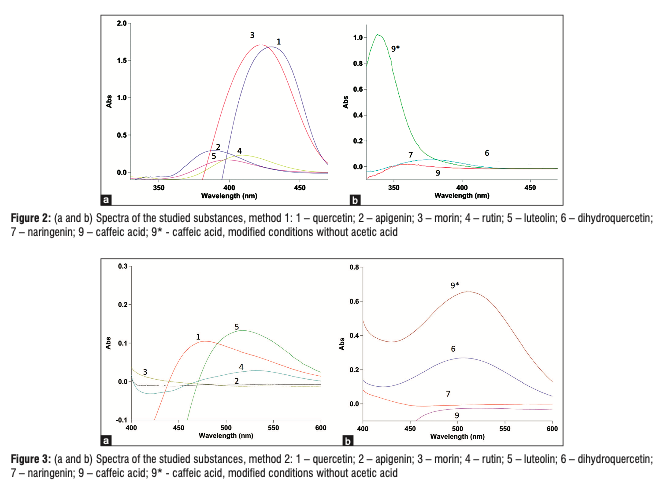
\includegraphics[width=\textwidth]{Flavonoid UV Results.png}
		\end{figure}
	\end{columns}

\end{frame}

\begin{frame}{Định lượng bằng phương pháp HPLC}
	Detertor: UV, FID, MS
	\begin{enumerate}
		\item Xây dựng phương pháp phân tích
		\begin{itemize}
			\item Thời gian lưu
			\item Hệ số phân giải
			\item Hệ số đối xứng
		\end{itemize}
		\item Thẩm định phương pháp phân tích
		\begin{itemize}
			\item Độ đặc hiệu (Tính chọn lọc) 
			\item Độ tích hợp hệ thống ($RSD$>2.0)
			\item Khoảng tuyến tính và đường chuẩn ($R^2$>0.995)
			\item Độ lặp lại ($RSD$>2.0) (Trong ngày và khác ngày)
			\item Độ thu hồi (Độ đúng) (Khác biệt với thuốc tây)
		\end{itemize}
	\end{enumerate}
	
\end{frame}
\section{Tác dụng sinh học của Flavonoid}
\mysectionpage
\begin{frame}{Tác dụng sinh học}
	\begin{itemize}
		\item Tác dụng như vitamin P làm biền thành mạch, giảm tính giòn và tăng tính thấm của mao mạch. Tác dụng được làm tăng khi kết hợp với acid ascorbic.
		\item Tác dụng chống oxy hóa: Do khả năng dọn gốc tự do, tạo phức với kim loại, ức chế phản ứng peroxy hóa lipid. Ngăn chặn nguy cơ xơ vữa đọng mạch, cao huyết áp, ung thư, stress, tiều đường và chống lão hóa.
		\item Bảo vệ gan khi gan bị tổn thương do một số độc chất.
		\item Tăng cường tuần hoàn động mạch và mao mạch: dành cho người bị rối loại trí nhớ.
		\item Tác dụng kháng khuẩn, kháng varus.
		\item Tác dụng chống ung thư do cơ chế chống oxy hóa 
		\item Chống dị ứng 
		\item Chống viêm loét và lành vết thương 
		\item Lợi tiểu 
		\item An thần 
		\item Diệt côn trùng
	\end{itemize}
\end{frame}
\section{Phân lập và Chiết xuất}
\mysectionpage
\begin{frame}{Phân lập và xác định cấu trúc}
	\begin{itemize}
		\item Không có phương pháp chung cho chiết xuất flavonoid vì tính tan khác nhau 
		\item Thường loại tạp chất bằng n-hexan sau đó chiết nóng bằng EtOH, MeOH.
		\item Tủ flavonodi bằng muối chì sau đó tác chì bằng cách sục dihydrosulfid
		\item Phân lập flavonoid bằng cột sắc ký
	\end{itemize}
\end{frame}
\begin{frame}{Chiết xuất và tinh chế quy mô công nghiệp}
	Không có phương pháp chung
	\begin{itemize}
		\item Chất tinh khiết  để làm thuốc 
		\item Chất tinh khiết để làm chất chuẩn 
		\item Cao dược liệu giàu hàm lượng hoạt chất 
		\item Cao dược liệu có hoạt tính sinh học
		\item Cao dược liệu chuẩn 
		\item Cao dược liệu định chuẩn 
	\end{itemize}
	Một số kỹ thuật chung 
	\begin{itemize}
		\item Chiết hồi lưu
		\item Chiết siêu âm 
		\item Chiết ngâm lạnh 
		\item Chiết siêu tới hạn
	\end{itemize}

\end{frame}
\section{Dược liệu chứa Flavonoid}
\mysectionpage
\begin{frame}
% Please add the following required packages to your document preamble:
% \usepackage{multirow}
% \usepackage{graphicx}
\begin{table}[]
	\resizebox{\columnwidth}{!}{%
	\begin{tabular}{llllll}
	\hline
	\multirow{2}{*}{Tên dược liệu} & \multicolumn{2}{c}{Dược điển} & \multirow{2}{*}{Tên dược liệu} & \multicolumn{2}{c}{Dược điển} \\ \cline{2-3} \cline{5-6} 
								   & Việt Nam       & Hồng kông    &                                & Việt Nam      & Hồng kông     \\ \hline
	{\bf Actiso}                         & X              &              & Bạch Quả                       &               & X             \\
	Cát căn                        & X              & X            & {\bf Cúc gai}                        & X             &               \\
	Mạch môn                       & X              & X & {\bf Chè dây}    & X             &               \\
	{\bf Hòe}                         & X (Nụ hoa)     & X(Quả)       & {\bf Xạ Can}                         & X             & X             \\
	{\bf Râu mèo}                        & X              &              & Dây mật                        &               &               \\
	{\bf Núc Nác}                       & X (Vỏ thân)    & X(Quả)       & {\bf Tô mộc}                         & X             &               \\
	{\bf Kim Ngân}                       & X              & X            & Chi {\bf Citrus}                     & X             & X             \\ \hline
	{\bf Dâu tằm} & X & X & {\bf Hoàng cầm} & X & X \\ 
	{\bf Diếp cá} & X & X & {\bf Bạch quả} & X & X \\  
	{\bf Kim tiền thảo} & X & X & {\bf Hồng hoa} & X & X \\ \hline
	\end{tabular}%
	}
	\end{table}
[1] Thông tư 06/VBHN-BYT về QUY ĐỊNH VỀ CHẤT LƯỢNG THUỐC, NGUYÊN LIỆU LÀM THUỐC
\end{frame}
\end{document}